% \documentclass[conference]{IEEEtran}
\documentclass[journal,onecolumn]{IEEEtran}
\IEEEoverridecommandlockouts
% The preceding line is only needed to identify funding in the first footnote. If that is unneeded, please comment it out.
% \usepackage{cite}
\usepackage{amsmath,amssymb,amsfonts}
\usepackage{algorithmic}
\usepackage{graphicx}
\usepackage[colorlinks=true, allcolors=blue]{hyperref}
\usepackage{url}
\usepackage{textcomp}
\usepackage{minted}
\usepackage{svg}
\usepackage{booktabs}
\usepackage{xcolor}
\usepackage[table]{xcolor}
\usepackage{colortbl}
\usepackage{multirow}
\usepackage{array}
\newcolumntype{C}[1]{>{\centering\arraybackslash}p{#1}}
\usepackage{adjustbox}
\usepackage{float}
\newminted{python}{
    linenos,
    autogobble,
    breaklines,
    fontsize=\scriptsize,
    frame=lines,
    framesep=2mm,
    bgcolor=black!5,
    rulecolor=\color{gray},
    framesep=3mm,
    baselinestretch=1.2,
    tabsize=4,
}
\usepackage[font=small,skip=0pt]{caption}
\captionsetup{skip=-0.001pt}
\usepackage{subcaption}
\captionsetup[subfigure]{aboveskip=-0.3pt}
\usepackage[style=apa,backend=biber]{biblatex}
\addbibresource{main.bib}
% Redefine macros for '&' symbol between two authors
\renewcommand*{\finalnamedelim}{%
  \ifnumgreater{\value{liststop}}{2}{\finalandcomma}{}%
  \addspace\&\space}
\def\BibTeX{{\rm B\kern-.05em{\sc i\kern-.025em b}\kern-.08em
    T\kern-.1667em\lower.7ex\hbox{E}\kern-.125emX}}

\begin{document}

\title{Comparative Analysis of Neural Network-Based Techniques for Vehicular Location Prediction}
%Proactive Vehicular Location Prediction for 5G Radio Resource Allocation Using Neural Network-Based Techniques}

\author{\IEEEauthorblockN{Sina Ebrahimi, \textit{SID: 13207801, Word Count: 3284}}\\
\IEEEauthorblockA{\textit{Centre for Future Transport and Cities} \\
\textit{Coventry University}\\
Coventry, UK \\
ebrahimis@coventry.ac.uk}
}

\maketitle

\begin{abstract}
Vehicular location prediction is crucial for improving Quality of Service (QoS) in fifth-generation (5G) radio Resource Allocation (RA). This study presents a novel comparison of five Neural Network (NN) models—Recurrent NN (RNN), Long Short-Term Memory (LSTM), Gated Recurrent Unit (GRU), one-dimensional convolutional NN (Conv1D), and Multi-Layer Perceptron (MLP)—in predicting vehicle positions using a dataset of vehicular mobility traces from Seoul, South Korea. The models are assessed using metrics such as coefficient of determination ($\text{R}^2$ score), Root Mean Square Error (RMSE), loss over epochs, and execution time per epoch. Out of the models tested, the MLP model showed the best performance, with an RMSE of 0.42 meters and an $\text{R}^2$ score of 0.999992. This represents a 32\% decrease in RMSE compared to Conv1D and the recurrent models and a significantly higher $\text{R}^2$ score. Moreover, MLP demonstrated the most rapid convergence and the shortest average execution time per epoch, emphasizing its efficiency. The results suggest that using simpler architectures, such as MLP, is quicker and more effective for this particular task. This provides valuable information for designing proactive RA strategies in 5G networks.
\end{abstract}

\begin{IEEEkeywords}
Prediction, Vehicular Mobility, Proactive Mobility Prediction, 5G, Handover Management, Radio Resource Management, Neural Networks
\end{IEEEkeywords}
\clearpage

\section{Introduction} \label{introduction}
%(5 marks) Should include the description of the chosen real-life problem and its significance (1-2 pages)
Fifth-generation (5G) wireless technology has enabled fast and responsive communication, which has greatly impacted sectors such as transportation. Especially in metropolitan areas, it is imperative to properly manage network resources for vehicle communications as vehicles are increasingly included in the Internet of Things (IoT) ecosystem. Radio Resource Management (RRM) is crucial in 5G networks as it optimizes network performance and guarantees Quality of Service (QoS) for users. Precise prediction of vehicle location can greatly improve RRM by facilitating proactive Resource Allocation (RA), enabling networks to allocate users to the most optimal base stations in advance of handovers (\cite{7931566}). This proactive approach is critical for properly controlling the always-shifting traffic patterns in urban areas because it can significantly reduce delays and improve connectivity.

Several Neural Network (NN) structures, including Recurrent NN (RNN), Long Short-Term Memory (LSTM), Gated Recurrent Unit (GRU), Convolutional NN (CNN), and Multi-Layer Perceptron (MLP), have demonstrated potential in forecasting intricate patterns (\cite{6795963,9204396}). Nevertheless, it is necessary to conduct a thorough analysis and evaluation of these architectures specifically in relation to vehicular location prediction for 5G RRM. This study aims to fill this void by assessing the efficacy of these NN architectures using vehicular mobility data obtained from Seoul, South Korea (\cite{dataset20kumbhar}). The models are assessed in terms of their computational efficiency, rate of convergence, and capacity to precisely forecast, offering insightful information on their appropriateness for real-time 5G applications. This work is distinctive in that it compares several NN architectures to enhance vehicle location predictions.

The next sections of this paper are organized as follows: Literature is briefly reviewed in Sec. \ref{related-work}. The problem and dataset are introduced in Sec. \ref{dataset}. The various NN-assisted methods utilized in this paper are succinctly introduced in Sec. \ref{methods}. Sec. \ref{results} presents the experimental results. Ultimately, discussion and future work are provided in Sec. \ref{discussions}.
\clearpage

\section{Related Work} \label{related-work}
% (10 marks) Should explain and properly cite the (most notable) works already done related to the selected problem. The references need to be from journal papers not just from websites.
The ability of vehicle location prediction to improve 5G radio performance has recently gained significant interest. While CNN-based models have also been shown to extract spatial features from this kind of data, LSTM networks have been shown to be successful in capturing temporal relationships in mobility data. ({\cite{9349962,7870510})). Within the context of 5G, scientists have looked at how Machine Learning (ML) methods might enhance network performance. Deep reinforcement learning techniques have specifically shown promise in optimizing joint mobility prediction and resource management (\cite{7725934,tvt23choi}).

ML algorithms have enhanced handover management in 5G networks, reducing service failures and thus greatly improving QoS (\cite{7792669,PRIYANKA2023100389}). Recent research suggests that simpler models such as MLP and one-dimensional convolutional NN (Conv1D) can occasionally achieve better performance than more complex recurrent architectures, especially in tasks involving spatio-temporal prediction. \cite{cikm23zhang} has demonstrated that MLP networks are successful in forecasting handovers in ultra-dense 5G networks, effectively managing intricate urban settings with exceptional precision and efficiency. Furthermore, Conv1D networks have demonstrated their efficacy in capturing localized patterns in sequential data, thus reinforcing the possibility of employing simpler models for mobility prediction tasks (\cite{7870510}).

These studies demonstrate the potential utility of NN-based techniques in determining the location of vehicles in 5G RRM. However, further investigation is required to comprehensively compare the various deep learning-based architectures. The objective of this study is to evaluate different architectures and identify the most suitable approach for proactive RA in 5G networks, thus addressing the existing gap in knowledge.
\clearpage

\section{Dataset} \label{dataset}
%  (10 marks) Should include the description of the publicly available dataset and its link (1-3 pages). Please describe the processes you use to clean and formalize the data set for your use.
The \texttt{vehicular mobility trace at Seoul, South Korea} dataset is accessed from IEEE DataPort (\cite{dataset20kumbhar}). The dataset is collected by simulating vehicles in urban environment using SUMO, which exports XML files as the raw output\footnote{Please refer to (\cite{sumo24fcd}) for the complete set of features.} (\cite{sumo24fcd}). The trace location in Seoul, South Korea has an area spanning over 2.5 × 1.5 km where there are are more than 30 intersections. A number of simulated vehicles are moving in the road topology. The dataset is introduced in a study regarding vehicular reliable routing that aims to select the routes with the longest connectivity time to efficiently deliver communication messages (\cite{lcomm21kumbhar}), where the authors introduced a heuristic to solve their problem. However, our goal is different, as we aim to predict the location of each vehicle in the next time step. We use the sparse scenario introduced in \cite{dataset20kumbhar} to conduct this experiment.

As part of the preprocessing stage, we initially transform the XML file \texttt{OpenStreetMap Trace for a Sparse Traffic.xml} into a CSV file. Then, we remove features \texttt{type, lane, slope, pos} as they do not influence vehicle mobility. We also convert the data type of the features \texttt{id} and \texttt{time} to integer to enhance readability and performance. The preprocessed features are shown in Table \ref{tab:features}. Moreover, Fig. \ref{fig:location} shows the coordinates of all vehicles across all the time steps in the environment. Overall, there are \textit{6 features and 1,483,385 records (comprising 3592 unique vehicles and 8220 time steps (seconds)}. 

Each time step might include some vehicles, and there is time dependency for the mobility of each individual vehicle throughout time steps. In order to predict the behavior of each vehicle, which is moving independently of the others, we generate sequences of length 5 for each vehicle by applying the \texttt{group by} method. Each sequence contains 4 features of x, y, angle, and speed for 5 consecutive time step for a unique vehicle followed by its location (x and y coordinates) at the fifth time step. We split the data with 80-20\% ratio between train and test datasets (detailed in Sec. \ref{preprocessing}).

\begin{table}[h!]
\centering
\begin{minipage}[t]{0.65\textwidth}
    \centering
    \scriptsize
    \caption{Dataset Features}
    \begin{tabular}{l|lp{1.8cm}lp{5.5cm}}
        Column & Data Type & Range & Unit & Description (\cite{dataset20kumbhar}) \\
        \hline
        \textbf{time} & Integer & 0 to 8219 & seconds & The time step described by the values within this timestep-element\\
        \textbf{id} & Integer & 0 to 4312 (3592 distinct vehicles) & - & The id of the vehicle\\
        \textcolor{blue}{\textbf{x}} & Float & 2.14 to 1420.58 & meters & (longitude) The absolute X coordinate of the vehicle (center of front bumper). The value depends on the given geographic projection \\
        \textcolor{blue}{\textbf{y}} & Float & 820.68 to 2212.71 & meters & (latitude) The absolute Y coordinate of the vehicle (center of front bumper). \\
        \textbf{angle} & Float & 0.0 to 360.0 & degrees & The angle of the vehicle in navigational standard (0-360 degrees, going clockwise with 0 at 12'o clock)\\
        \textbf{speed} & Float & 0.0 to 37.38 & m/s & The speed of the vehicle\\
    \end{tabular}
    \label{tab:features}
    \captionsetup{singlelinecheck=false, justification=raggedright}
    \caption*{\centering \footnotesize *The blue features are the subject of prediction for individual vehicles.}
    \vspace{-5mm}
\end{minipage}%
\hfill
\begin{minipage}[t]{0.32\textwidth}
    \centering
    \caption{Hyperparameter Grid for Tuning}
    \label{tab:tuning-values}
    \begin{tabular}{c|p{2.5cm}}
    \textbf{Hyperparameter} & \textbf{Values} \\
    \hline
    Hidden Size & 50, 100 \\
    No. of Layers & 2, 3, 4 \\
    Learning Rate & 0.1, 0.05, 0.01, 0.005, 0.001, 0.0005, 0.0001, 0.00005 \\
    No. of Epochs & 30 \\
    \end{tabular}
\end{minipage}
\end{table}
\clearpage

\section{Methods} \label{methods}
% (15 marks) Should describe the appropriate neural network(s), together with the learning algorithm(s) and other parameters, tried to solve the problem. Please provide the reasoning behind selecting the type of the neural network and parameters.
This section explains the fundamental models employed for predicting vehicle movement, focusing on RNN, LSTM, GRU, Conv1D, and MLP. Each model is chosen for its ability to capture temporal and spatial patterns in sequential data.

\subsection{RNN}
RNNs are designed for sequential data processing, utilizing a looped structure to retain information from previous time steps. This makes them suitable for tasks like time-series forecasting and vehicle movement prediction, where temporal data sequence is key.

The RNN architecture consists of:
\begin{itemize}
    \item \textbf{Input Layer:} Receives sequential data as input vectors at each time step.
    \item \textbf{Hidden Layers:} Feature recurrent connections, allowing the network to preserve information over time. The hidden state \( h_t \) at time step \( t \) is calculated as:
    \[
    h_t = \sigma(W_{xh} \cdot x_t + W_{hh} \cdot h_{t-1} + b_h)
    \]
    where \( x_t \) is the input at \( t \), \( W_{xh} \) and \( W_{hh} \) are the weight matrices, \( b_h \) is the bias vector, and \( \sigma \) denotes the activation function (e.g., tanh or ReLU\footnote{ReLU is chosen in our RNN method due to its flexibility in remembering states.}).
    \item \textbf{Output Layer:} Generates the output \( y_t \) for the current time step:
    \[
    y_t = \sigma(W_{hy} \cdot h_t + b_y)
    \]
    where \( W_{hy} \) represents the weight matrix that connects the hidden state to the output, and \( b_y \) is the bias vector.
\end{itemize}

RNNs are foundational for sequence modeling but can struggle with long-term dependencies due to vanishing gradients, making them better suited for short-term predictions (\cite{prep23ghojogh}).

\subsection{LSTM}
LSTM networks extend RNNs by incorporating memory cells and gating mechanisms to handle long-term dependencies effectively (\cite{6795963}). This makes them ideal for tasks requiring the retention of information over extended periods, like predicting vehicle trajectories based on historical data.

The LSTM architecture includes:
\begin{itemize}
    \item \textbf{Input Layer:} Sequential data enters the network at each time step.
    \item \textbf{LSTM Cells:} Each cell contains forget (\( f_t \)), input (\( i_t \)), and output  (\( o_t \)) gates, which manage the flow of information:
    \[
    f_t = \sigma(W_f \cdot [h_{t-1}, x_t] + b_f) \qquad \qquad i_t = \sigma(W_i \cdot [h_{t-1}, x_t] + b_i)
    \]
    \[
    \tilde{C}_t = \tanh(W_C \cdot [h_{t-1}, x_t] + b_C) \qquad \qquad C_t = f_t \cdot C_{t-1} + i_t \cdot \tilde{C}_t
    \]
    \[
    o_t = \sigma(W_o \cdot [h_{t-1}, x_t] + b_o) \qquad \qquad h_t = o_t \cdot \tanh(C_t)
    \]
    where \( C_t \) is the cell state.
    \item \textbf{Output Layer:} The final hidden state generates the prediction, which represents the next position of the vehicle.    
\end{itemize}

LSTMs are selected for their robustness in modeling complex temporal sequences, making them suitable for long-term vehicle trajectory prediction.

\subsection{GRU}
GRUs simplify the LSTM architecture by merging the input and forget gates into a single update gate, reducing complexity and computational cost while still capturing long-term dependencies (\cite{prep23ghojogh}).

The GRU architecture features:
\begin{itemize}
    \item \textbf{Input Layer:} Sequential data is fed into GRU cells at each time step.
    \item \textbf{GRU Cells:} Comprising reset (\( r_t \)) and update (\( z_t \)) gates that regulate information flow:
    \[
    r_t = \sigma(W_r \cdot [h_{t-1}, x_t] + b_r)  \qquad \qquad z_t = \sigma(W_z \cdot [h_{t-1}, x_t] + b_z)
    \]
    \[
    \tilde{h}_t = \tanh(W_h \cdot [r_t \cdot h_{t-1}, x_t] + b_h)  \qquad \qquad h_t = z_t \cdot h_{t-1} + (1 - z_t) \cdot \tilde{h}_t
    \]
    where \( \tilde{h}_t \) represents the candidate activation, and \( h_t \) is the updated hidden state.
    \item \textbf{Output Layer:} Generates the final prediction from \( h_t \).
\end{itemize}

GRUs are chosen for their efficiency and performance in tasks where both precision and computational resources are critical.

\subsection{Conv1D}
Conv1D models are used to analyze sequential data, utilizing convolutional filters to capture spatial hierarchies, making them effective for identifying local patterns in vehicle trajectory data (\cite{jymssp21kiranyaz}).

The Conv1D architecture includes:
\begin{itemize}
    \item \textbf{Input Layer:} The input data consists of sequences representing time-varying features, which are flattened before being fed into the input layer.
    \item \textbf{Convolutional Layers:} Conv1D layers utilize a collection of convolutional filters to process the input sequence. The filters move across the input, capturing specific characteristics in the surrounding area:
    \[
    z_t = \sum_{i=1}^{k} w_i \cdot x_{t+i-1} + b
    \]
    where \( k \) is the kernel size, \( w_i \) are the filter weights, and \( b \) is the bias term.
    \item \textbf{Pooling Layers:} Reduce dimensionality, typically using max pooling to retain key features.
    \item \textbf{Fully Connected (Dense) Layer:} Aggregates features to produce the final output.
\end{itemize}

Conv1D models excel at capturing local dependencies, providing an alternative to recurrent networks by emphasizing local feature extraction.

\subsection{MLP}
MLPs are feedforward NNs consisting of multiple layers of interconnected neurons, capable of learning complex, non-linear relationships between input features and output predictions (\cite{cikm23zhang}).

The MLP architecture comprises:
\begin{itemize}
    \item \textbf{Input Layer:} Receives flattened sequential data.
    \item \textbf{Hidden Layers:} Each layer \( l \) performs a weighted sum of inputs followed by a non-linear activation function (i.e. ReLU):
    \[
    h^{(l)} = \sigma(W^{(l)} \cdot h^{(l-1)} + b^{(l)})
    \]
    where \( h^{(l)} \) is the output of the \( l \)-th layer, \( W^{(l)} \) is the weight matrix, and \( b^{(l)} \) is the bias vector.
    \item \textbf{Output Layer:} Provides the predicted output.
\end{itemize}

Although MLPs do not explicitly incorporate temporal dependencies, they can be utilized for predicting vehicle movement by considering the sequential data as a collection of features. This allows for the learning of non-linear relationships between past movements and future positions. MLPs are employed as a reference model to evaluate the influence of integrating temporal structures in prediction tasks. They offer a direct method for modeling relationships within the data, acting as a benchmark for more intricate models such as RNNs, LSTMs, and Conv1D networks.

Fig. \ref{fig:nn-architecture} illustrates a generic architecture for all the methods, assuming the presence of three layers, each consisting of 50 neurons. The depicted diagram resembles MLPs and does not illustrate the complexities of other techniques (such as the forget gate in LSTM), despite the fact that all these methods have the same number of layers and neurons. For more detailed information about the models (e.g., utilized activation functions), please refer to step 3 in Sec. \ref{tuning-annex}.

%%%%%%%%%%%%%%%%%%%%
\section{Experimental Results} \label{results}
%(15 marks) Should explain the rigor experiments conducted and compare their detailed results.
The experiments were carried out using PyTorch and widely used Python libraries on a High-Performance Computing (HPC) node at Coventry University called \texttt{zeus400}. This node is equipped with an NVIDIA Tesla K80 GPU. This section provides an overview of the metrics utilized for comparing models, the process of tuning hyperparameters, and the comparative analysis of the five NN-based techniques based on the chosen hyperparameters.

\subsection{Metrics}
The efficacy of the location prediction models was assessed using fundamental metrics: Root Mean Square Error (RMSE), Mean Absolute Error (MAE), and the coefficient of determination ($\text{R}^2$ score). In addition, we monitored the loss function throughout the epochs and documented the average time it took to complete each epoch.

\paragraph{RMSE}
is a metric that measures the magnitude of the differences between predicted and actual values. It emphasizes larger errors by squaring the discrepancies. Smaller RMSE values indicate higher model accuracy (\cite{cr05willmott}). The study emphasizes the significance of RMSE as it offers a quantitative assessment of the overall precision of the models' predictions. Smaller RMSE values indicate better performance of the models.

\paragraph{MAE}
is a metric that calculates the average of the absolute differences between predicted and actual values. It provides a straightforward measure of prediction error without giving more importance to larger errors. It provides additional information to RMSE by giving a better understanding of the accuracy of predictions, especially in terms of the typical sizes of errors (\cite{cr05willmott}).

\paragraph{$\text{R}^2$ Score}
quantifies the amount of variability in the dependent variable that can be explained by the model. A higher value, with a maximum of 1, indicates a more robust correlation with the data. It is crucial to comprehend the model's ability to explain things effectively (\cite{biomet91nagelkerke}).

\paragraph{Loss}
was monitored throughout all epochs to assess the convergence and stability of the model during training. Lower loss values suggest better model performance in fitting the training data (\cite{mit16goodfellow}).

\paragraph{Average Execution Time per Epoch}
is important for assessing computational efficiency, helping balance accuracy with time constraints in practical applications (\cite{jproc17sze}).

\subsection{Hyperparameter Tuning}
Optimizing NN model performance requires thorough hyperparameter tuning (\cite{mit16goodfellow}). We analyzed different arrangements using a hyperparameter grid (Table \ref{tab:tuning-values}).

The grid search resulted in 48 unique combinations of hyperparameters, enabling a thorough examination of the hyperparameter space to determine the most optimal configurations for each model (e.g., LSTM). To accelerate the process, we evaluated each combination using 10\% of the training and test datasets. The RMSE and $\text{R}^2$ scores for each method were assessed using the specified hyperparameter combinations, and a ranking system was developed to identify the optimal combination for each method, as detailed in Sec. \ref{tuning-annex}. The hyperparameter sets selected for final analysis are highlighted in green in Table \ref{tab:top-experiments-tuning}.

\begin{table}[htbp]
\centering
\caption{Top Experiments for Each Method}
\label{tab:top-experiments-tuning}
\resizebox{\textwidth}{!}{%
\begin{tabular}{C{1.2cm}C{0.7cm}C{1.1cm}C{1.2cm}C{1cm}C{1cm}C{1.5cm}C{1.7cm}C{1cm}C{1cm}C{1cm}}
\hline
\textbf{Method} & \textbf{Hidden Size} & \textbf{No. of Layers} & \textbf{Learning Rate ($\alpha$)} & \textbf{RMSE} & \textbf{MAE} & \textbf{$\text{R}^2$ Score} & \textbf{Avg Epoch Time} & \textbf{Final Loss} & \textbf{Final Epoch} & \textbf{Combined Rank} \\
\hline
\multirow{3}{*}{\textbf{RNN}} & \rowcolor{green!30} 100 & 2 & 0.0005 & 16.26 & 11.05 & 0.9890 & 18.12 & 115.46 & 30 & 7.5 \\
 & 100 & 2 & 0.001 & 59.52 & 41.63 & 0.8712 & 18.25 & 3824.85 & 30 & 11.9 \\
 & 100 & 2 & 0.05 & 180.51 & 126.69 & -0.0470 & 18.2 & 35930.73 & 5 & 53.1 \\ \hline
\multirow{3}{*}{\textbf{LSTM}} & \rowcolor{green!30} 100 & 4 & 0.0005 & 10.8 & 6.68 & 0.9959 & 23.69 & 53.01 & 30 & 8.2 \\
 & 100 & 2 & 0.0005 & 10.76 & 7.3 & 0.9956 & 20.525 & 67.74 & 30 & 10.525 \\
 & 100 & 2 & 0.001 & 12.49 & 8.39 & 0.9947 & 20.39 & 213.96 & 30 & 18.52 \\ \hline
\multirow{3}{*}{\textbf{GRU}} & \rowcolor{green!30} 100 & 3 & 0.0005 & 10.68 & 6.84 & 0.9962 & 22.88 & 104.95 & 30 & 8.07 \\
 & 100 & 2 & 0.0005 & 14.43 & 10.81 & 0.9933 & 21.95 & 96.07 & 30 & 11.26 \\
 & 50 & 3 & 0.001 & 16.68 & 10.71 & 0.9901 & 21.16 & 410.59 & 30 & 16.94 \\ \hline
\multirow{3}{*}{\textbf{Conv1D}} & \rowcolor{green!30} 50 & 3 & 0.0001 & 0.62 & 0.37 & 0.999985 & 18.44 & 0.83 & 30 & 26.45 \\
 & 50 & 3 & 0.0005 & 0.525 & 0.4 & 0.999991 & 18.45 & 1.9 & 30 & 28.35 \\
 & 50 & 2 & 0.0001 & 0.78 & 0.5 & 0.999976 & 16.73 & 0.67 & 30 & 32.2 \\ \hline
\multirow{3}{*}{\textbf{MLP}} & \rowcolor{green!30} 100 & 3 & 0.00005 & 0.42 & 0.23 & 0.999992 & 15.78 & 0.36 & 30 & 7.34 \\
 & 50 & 2 & 0.0001 & 0.525 & 0.41 & 0.999990 & 14.3 & 0.35 & 30 & 16.2 \\
 & 100 & 2 & 0.0001 & 0.525 & 0.36 & 0.999988 & 14.41 & 0.38 & 30 & 18.0 \\
\hline
\end{tabular}}
\end{table}
\clearpage

\subsection{Methods Comparison} \label{sec-comparison}
Several NN architectures—RNN, LSTM, GRU, Conv1D, and MLP—are compared in this part. Using the previously mentioned metrics helps one evaluate the performance. The further study is based on the ideal hyperparameter configuration for every method, shown by the green highlighting in Table \ref{tab:top-experiments-tuning}. It is crucial to mention that when predicting vehicle positions (x and y coordinates), the units for RMSE, MAE, and loss (calculated using MSE) are expressed in meters (m).

\paragraph{Visualizing predicted locations}
Fig. \ref{fig:pred-vs-actual-all-vehicles} displays the projected and real positions of all vehicles throughout all time intervals for all the utilized techniques. The predictions made by MLP and Conv1D closely align with the actual locations, whereas RNN fails to accurately detect vehicle locations. Nevertheless, the graph is excessively congested to analyze. Hence, in Figs. \ref{fig:pred-vs-actual-random-vehicle-1} and \ref{fig:pred-vs-actual-random-vehicle-2}, we examine the paths of two random vehicles over a period of time for a more detailed analysis. The forecasting performed by Conv1D and MLP techniques is exceptional. Nevertheless, the LSTM and GRU methods fail to accurately predict the locations of some of the sampled vehicles. Furthermore, the RNN method exhibits significant disparities between actual and predicted locations.

\paragraph{RMSE, MAE, and $\text{R}^2$ Score Comparison}
As depicted in Fig. \ref{fig:rmse-mae-r2-methods}, the MLP model surpasses all other methods in terms of the important metrics. The achieved RMSE is 0.42 meters, which is roughly 32\% lower than the RMSE of the second-best Conv1D model, which is 0.62 meters. In addition, the MLP model achieves an MAE of 0.23 meters, which is 38\% superior to the Conv1D model's MAE of 0.37 meters. The coefficient of determination ($\text{R}^2$) score for the MLP model is likewise the highest, reaching 0.999992. This value suggests an almost flawless level of prediction accuracy. This demonstrates the exceptional aptitude of MLP in precisely predicting vehicle positions with remarkable accuracy and a minimal error margin.

Although MLP outperforms Conv1D, Conv1D still shows strong performance with an RMSE of 0.62 meters and an MAE of 0.37 meters. On the other hand, the conventional recurrent models (RNN, LSTM, and GRU) demonstrate considerably higher RMSE and MAE values, with RNN doing the poorest. For example, the RMSE of the RNN is 16.26 meters, which is almost 38.7 times greater than the RMSE of the MLP. The notable disparity underscores the constraints of basic recurrent architectures in comprehending the intricate dynamics of vehicle movements compared to more straightforward models such as MLP and Conv1D.

\paragraph{Loss Over Epochs}
Convergence pertains to the speed and efficiency at which the loss function of each model reaches a stable minimum value during the training phase. As seen in Fig. \ref{fig:loss-over-epochs}, the MLP method shows the fastest and most constant convergence. Its loss from 6248.56 in the first epoch to roughly 0.11 by the 27th epoch clearly shows effective learning with almost no oscillations. Although the Conv1D approach has a slower pace, it exhibits satisfactory convergence, reaching a loss of around 3.45 by the 11th epoch and maintaining stability. These findings indicate that simpler models like MLP and Conv1D may optimize their weights more efficiently, rendering them highly effective for this particular task.

On the other hand, LSTM and GRU exhibit slower and less consistent convergence, reaching final losses of 22.59 and 174.87, respectively, by the 30th epoch. The GRU approach required only 12 epochs to complete and did not require further progression. The RNN model demonstrates the most significant challenge, as evidenced by its highest ultimate loss of 174.87. This indicates difficulties in accurately identifying the fundamental patterns within the data. The RNN model attained its minimum recorded loss of 116.77 meters in the 10th epoch. LSTM and GRU, despite their theoretical advantages for sequential data, necessitate a greater number of epochs for complete optimization and display more volatility during training due to their intricate structures. This investigation demonstrates that MLP and Conv1D not only produce lower loss values, but they also do it more effectively, rendering them more appropriate for this particular location prediction task.

\paragraph{Execution Time Per Epoch}
With the Conv1D model closely behind, Fig. \ref{fig:exec-time-over-epochs} shows that the MLP model displays the lowest average execution time per epoch. MLP's simplicity—that which includes fully connected layers free from sequential processing—helps to explain its computational efficiency. More effective than other methods is Conv1D, which employs convolutional operations. This results from the slower stride used for pooling layers, which guarantees accuracy while accelerating data processing.

On the other hand, recurrent models, specifically LSTM and GRU, have longer execution times per epoch. The LSTM model, for instance, has an average epoch duration of 23.69 seconds, which is over 50\% longer than the MLP model's 15.78 seconds. The longer execution time is due to the complexity of the LSTM and GRU architectures. They have to process sequential data and keep hidden states between time steps, which makes them harder to compute.
\clearpage

\section{Discussion and Future Work} \label{discussions}
% (5 marks) Should present the summary of the findings (1-2 pages). Also provide what future work can be conducted on this project.
MLP emerged as the best-performing model in all categories, combining high prediction accuracy with excellent computational efficiency. Conv1D also demonstrated strong and consistent performance, making it a viable choice. While RNN, LSTM, and GRU are theoretically advantageous for sequence modeling, they are less suitable for accurate and efficient vehicle location prediction in this context.

The differences in architecture between these models are most likely to explain the findings. The MLP's fully connected layers are ideal for the small input size and specific nature of this prediction task, allowing it to reach high precision quickly. Conv1D's convolutional layers accurately capture spatial relationships, yielding high precision and short wall-clock times. On the other hand, the iterative nature of RNN, LSTM, and GRU, though beneficial in some sequential tasks, adds unnecessary complexity for this particular forecasting application. 

Our study indicates that MLP and Conv1D models outperform traditional recurrent models (RNN, LSTM, GRU) in vehicular location prediction for 5G RRM. The MLP model performed particularly well on metrics such as $\text{R}^2$ score, RMSE, MAE, and computational efficiency. These findings call into question the widespread belief that recurrent models are always superior for sequential data handling. Instead, they propose that simpler architectures like MLP and Conv1D might work better for some prediction tasks. These architectures offer faster training and inference times, which are important for real-time 5G applications, while still being able to capture patterns in space and time.

Future research should prioritize the integration of these models into a proactive 5G RRM framework. This integration should make use of their predictive capabilities to optimize network resources by taking into account the expected positions of vehicles. Furthermore, investigating hybrid models that integrate the advantages of MLP, Conv1D, and recurrent architectures could improve prediction accuracy in more intricate settings. Additional research should evaluate the ability of these models to be expanded and applied in larger and denser urban settings, as well as their effectiveness in different traffic situations. Evaluating the models' capacity to adapt to changing mobility patterns and resilience to different data sampling rates would give substantial insight for practical application. Incorporating effective location prediction into 5G RRM enables the development of intelligent, user-centric networks capable of consistently delivering QoS in extremely mobile environments.
\clearpage

% \bibliographystyle{ieeetr} 
% \bibliography{main}{}

% Where you want the bibliography to appear
\printbibliography % References (5 marks) List of references cited in the other sections, in the APA style
\clearpage

\begin{appendices}

\section{Screenshots and Steps} \label{appendix-steps}
%Appendix 1- Screenshots and steps (15 marks) Should contain the screenshots of all the steps together with brief descriptions such that an interested reader can re-do all the experiments in this research.
The graphs from the report are appeared in this section.

\begin{figure}[H]
    \centering
    \begin{subfigure}[b]{0.46\linewidth}
        \centering
        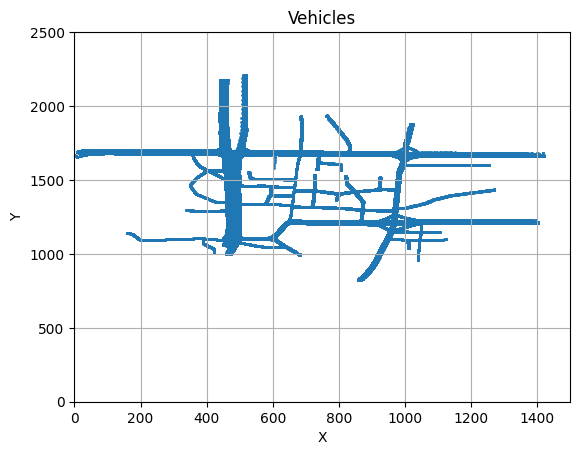
\includegraphics[width=\linewidth]{figures/location.png}
        \caption{}
        \label{fig:location}
    \end{subfigure}%
    \begin{subfigure}[b]{0.54\linewidth}
        \centering
        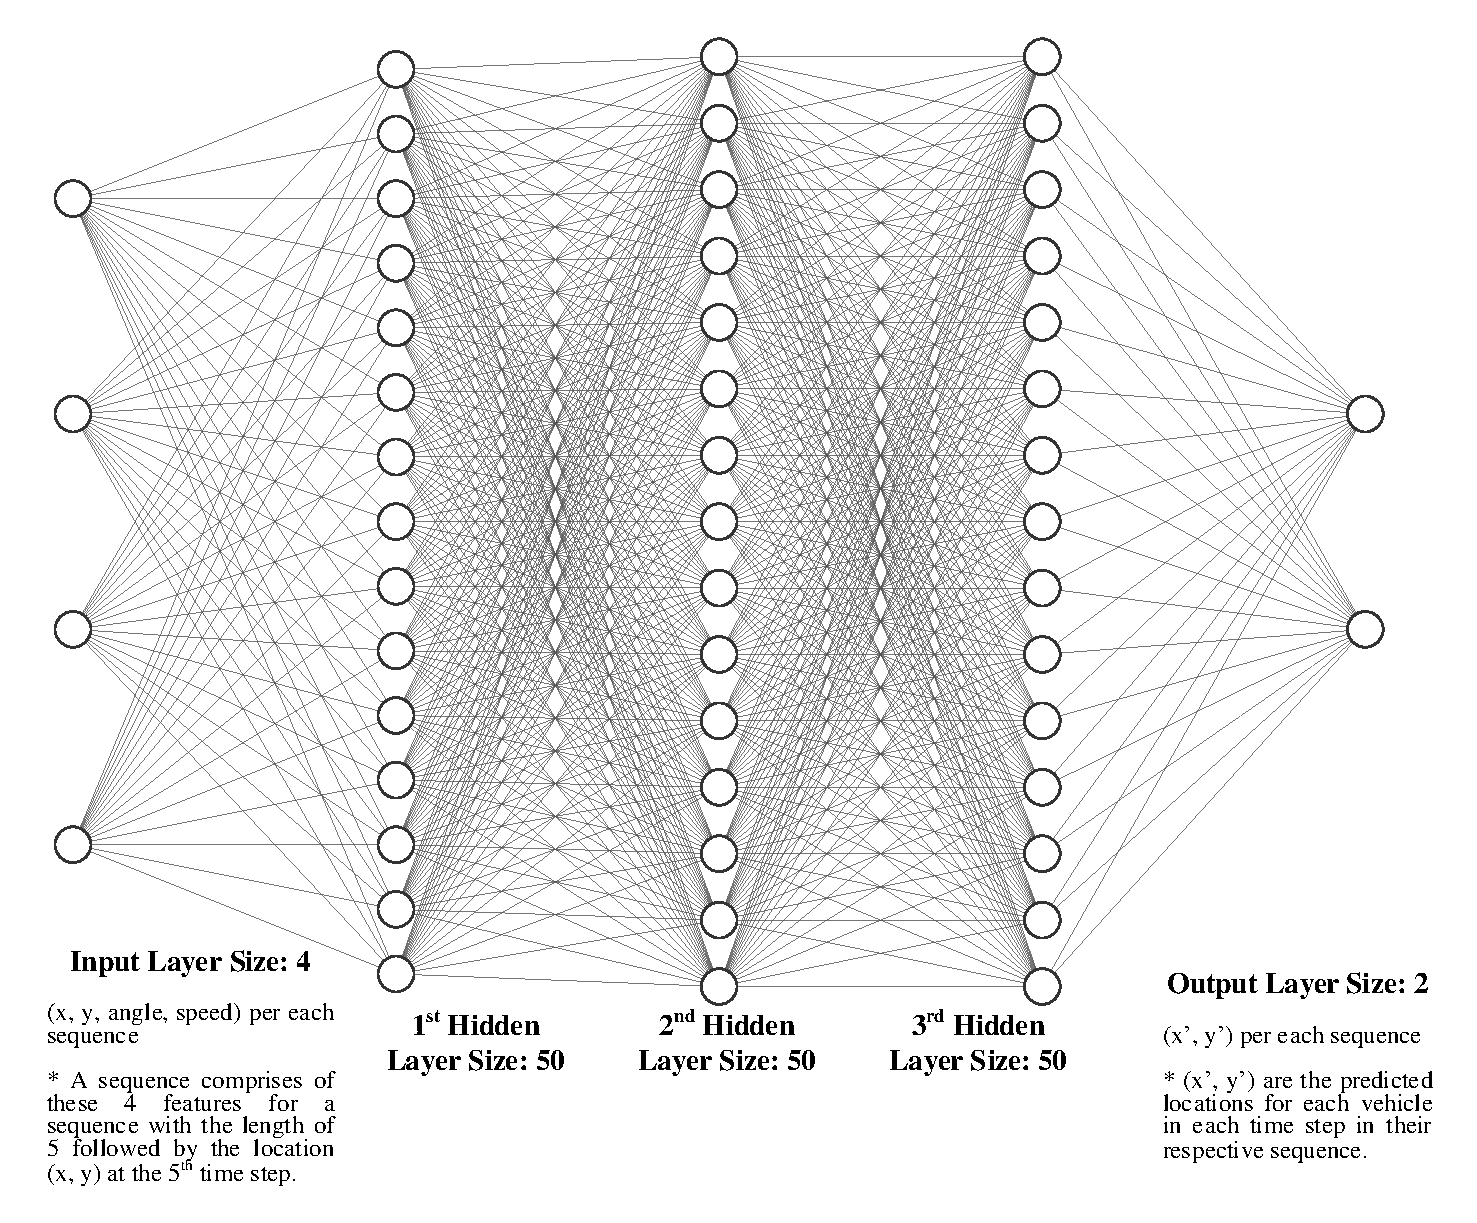
\includegraphics[width=\linewidth]{figures/architecture.pdf}
        \caption{}
        \label{fig:nn-architecture}
    \end{subfigure}
    \caption{a) Location of all vehicles throughout all time steps (\cite{dataset20kumbhar}), b) Generic NN architecture (Image generated using (\cite{joss19lenail})).}
    \label{fig:side-by-side}
\end{figure}


\begin{figure}[H]
    \centering
    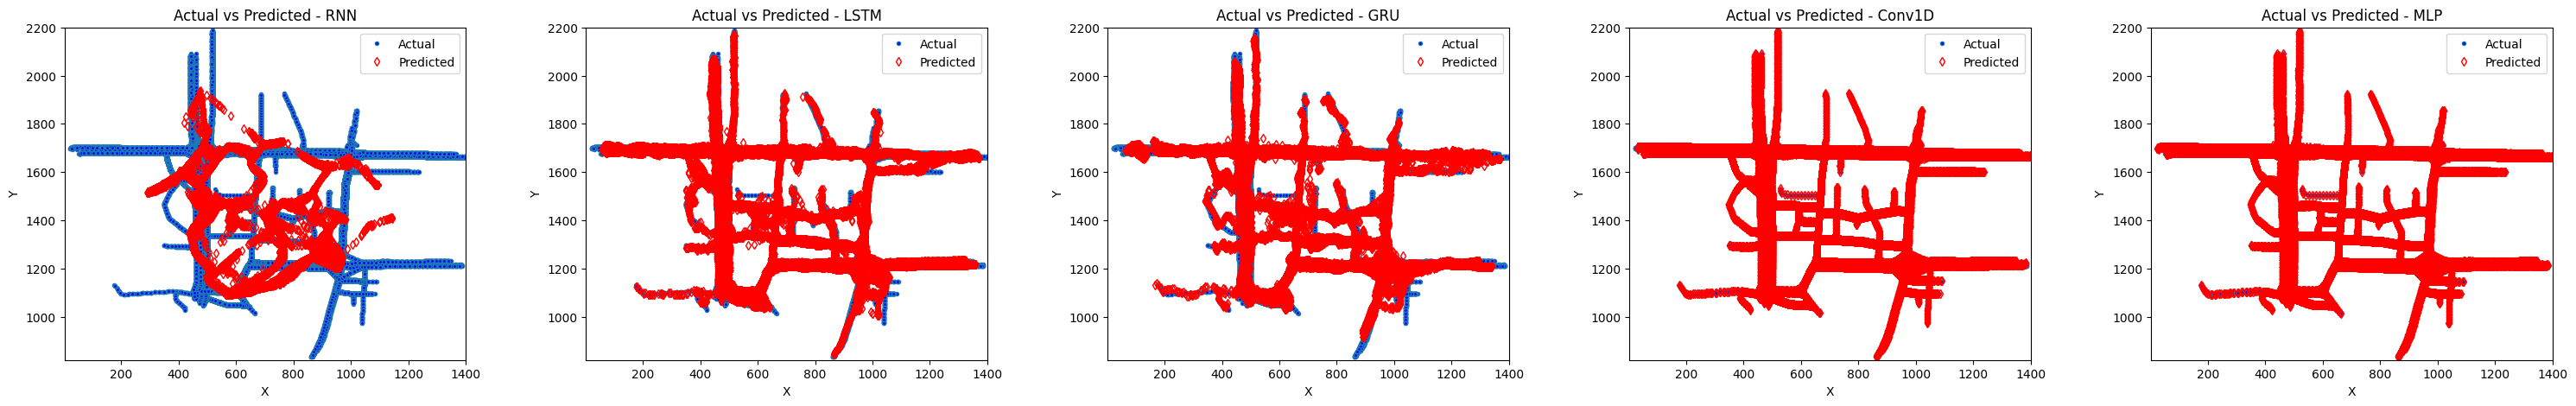
\includegraphics[width=1\textwidth]{figures/all_vehicles_comparison.png}
    \caption{Visualization of predicted and actual locations for all vehicles across all time steps using five different methods.}
    \label{fig:pred-vs-actual-all-vehicles}
\end{figure}

\begin{figure}[H]
    \centering
    \includesvg[width=1\textwidth]{figures/vehicle_4225_comparison.svg}
    \caption{Visualization of predicted and actual locations for a random vehicle across all time steps using five different methods (1).}
    \label{fig:pred-vs-actual-random-vehicle-1}
\end{figure}

\begin{figure}[H]
    \centering
    \includesvg[width=1\textwidth]{figures/vehicle_3726_comparison.svg}
    \caption{Visualization of predicted and actual locations for a random vehicle across all time steps using five different methods (2).}
    \label{fig:pred-vs-actual-random-vehicle-2}
\end{figure}

\begin{figure}[H]
    \centering
    \includesvg[width=1.03\textwidth]{figures/rmse-mae-r2score-methods.svg}
    \caption{RMSE, MAE, and $\text{R}^2$ score of the final epoch for various methods.}
    \label{fig:rmse-mae-r2-methods}
\end{figure}

\begin{figure}[H]
    \centering
    \begin{subfigure}[b]{0.45\linewidth}
        \centering
        \includesvg[width=\textwidth]{figures/loss-over-epochs.svg}
        \caption{}
        \label{fig:loss-over-epochs}
    \end{subfigure}%
    \begin{subfigure}[b]{0.6\linewidth}
        \centering
        \includesvg[width=\textwidth]{figures/exec-time-per-epoch.svg}
        \caption{}
        \label{fig:exec-time-over-epochs}
    \end{subfigure}
    \caption{a) Loss (based on MSE) and b) average execution time (s) per epoch for different methods.}
    \label{fig:methods-comparison}
\end{figure}
\clearpage

Experiments were conducted on a Coventry University HPC node (\texttt{zeus400}) equipped with an NVIDIA Tesla K80 GPU (24GB GDDR5, comprising two NVIDIA GK210 GPUs), an Intel Xeon E5-2683 v4 CPU @ 2.10GHz with 32 cores, and 128 GB of RAM. The system runs a GNU/Linux operating system with kernel version 4.18, utilizing CUDA version 11.4 and Nvidia driver version 470.199.02. In the folder \texttt{ann\_project}, a new Python virtualenv is created, and the following packages are installed:

\begin{minted}[fontsize=\footnotesize, linenos, breaklines, bgcolor=black!5]{bash}
[ebrahimis@zeus400 ~]$ module load python/last
[ebrahimis@zeus400 ~]$ module load cuda/last
[ebrahimis@zeus400 ~]$ module load gcc/gcc
[ebrahimis@zeus400 ~]$ cd ann_project/
[ebrahimis@zeus400 ann_project]$ python3 --version
Python 3.8.8
[ebrahimis@zeus400 ann_project]$ python -m venv venv
[ebrahimis@zeus400 ann_project]$ source venv/bin/activate
(venv) [ebrahimis@zeus400 ann_project]$ pip install pandas numpy torch scikit-learn matplotlib
(venv) [ebrahimis@zeus400 ann_project]$ code .
\end{minted}

\begin{figure}
    \centering
    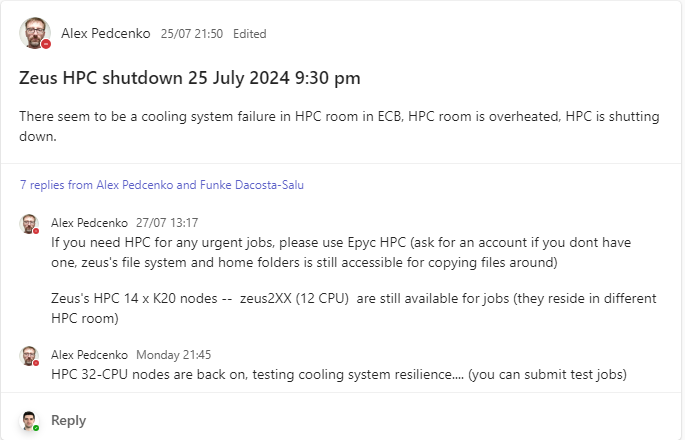
\includegraphics[width=0.59\linewidth]{figures/scr-0-zeus.png}
    \caption{Downtime of Zeus nodes.}
    \label{fig:scr-0-zeus}
\end{figure}

Unfortunately, the Zeus nodes have been non-operational since July 25th, 2024, and they remain inactive as of today's date, August 5th, 2024 (see Fig. \ref{fig:scr-0-zeus}). Although initial experiments with LSTM and some hyperparameter tuning were performed on Zeus nodes (no captured screenshots at the time), the majority of the results were obtained using Google Colab. Displayed below are screenshots depicting the concluding phase of the training process on an MLP model (Figs. \ref{fig:scr-1-colab}, \ref{fig:scr-2-colab}, \ref{fig:scr-3-colab}, and \ref{fig:scr-4-colab}). The detailed code of the notebooks can be found in Sec. \ref{appendix-code}. An interested reader can re-run all the experiments using the existing code.

\begin{figure}
    \centering
    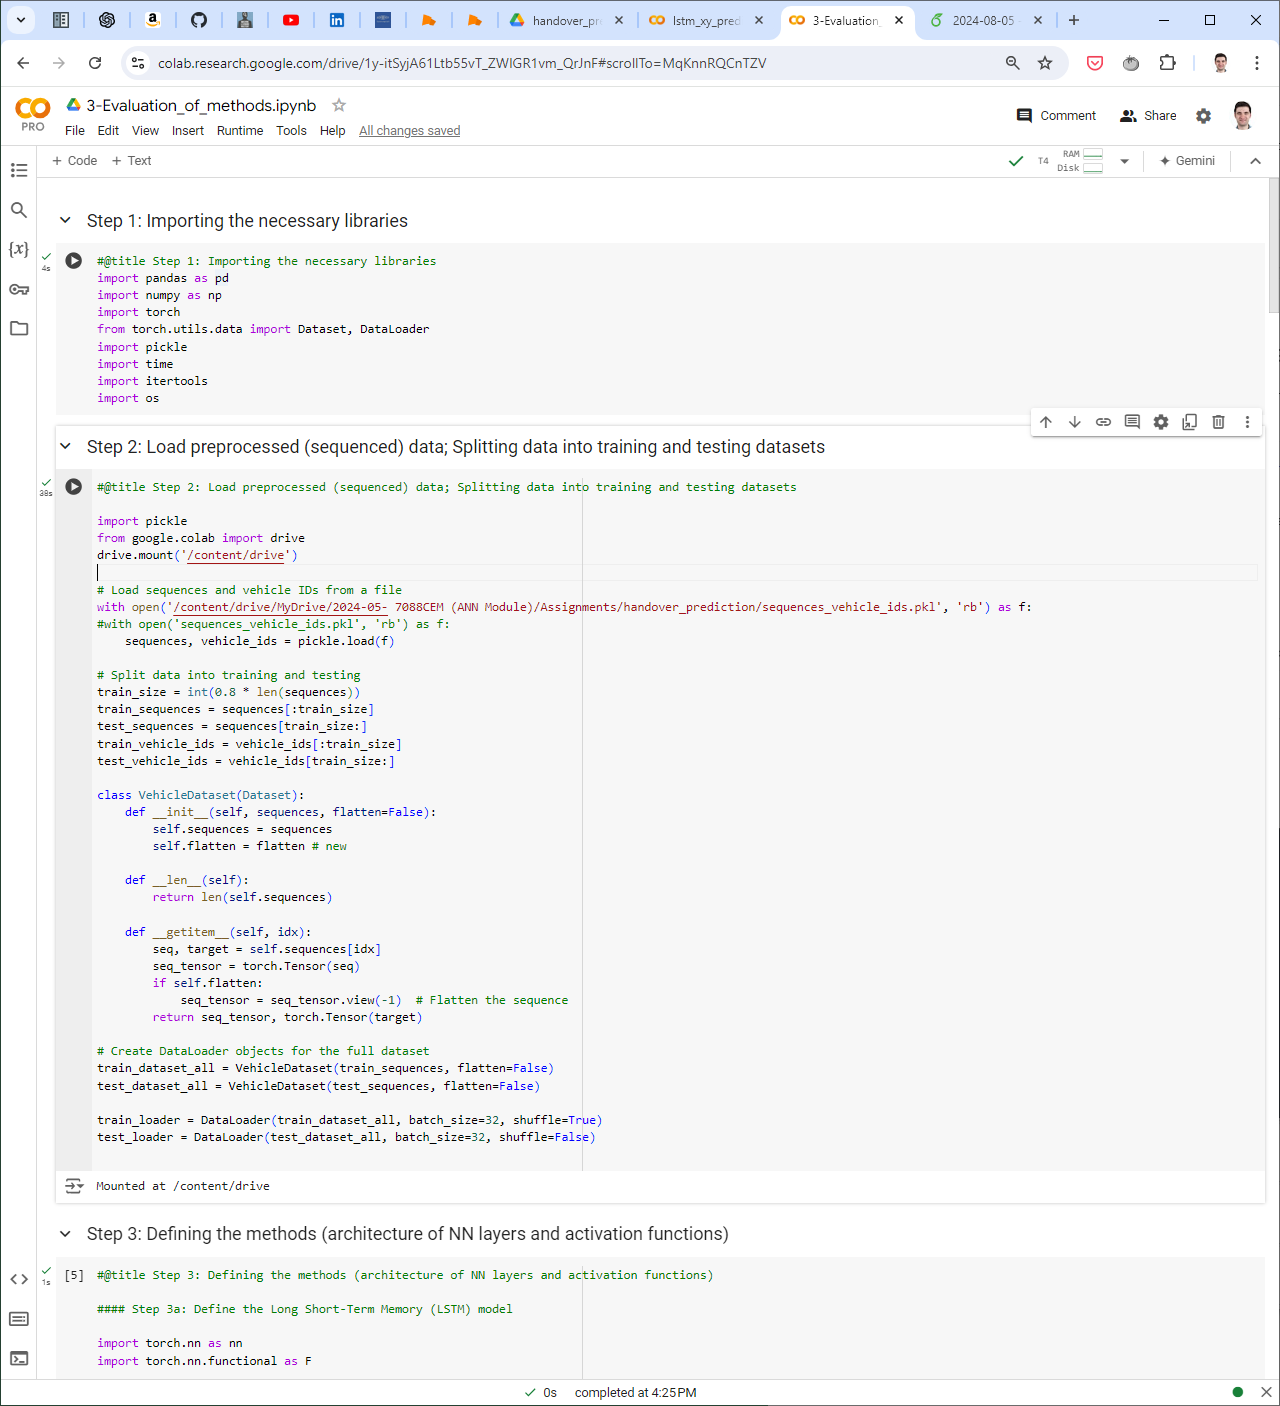
\includegraphics[width=0.99\linewidth]{figures/scr-1-colab.png}
    \caption{Steps 1 and 2: importing libraries, reading the dataset, and splitting the data.}
    \label{fig:scr-1-colab}
\end{figure}

\begin{figure}
    \centering
    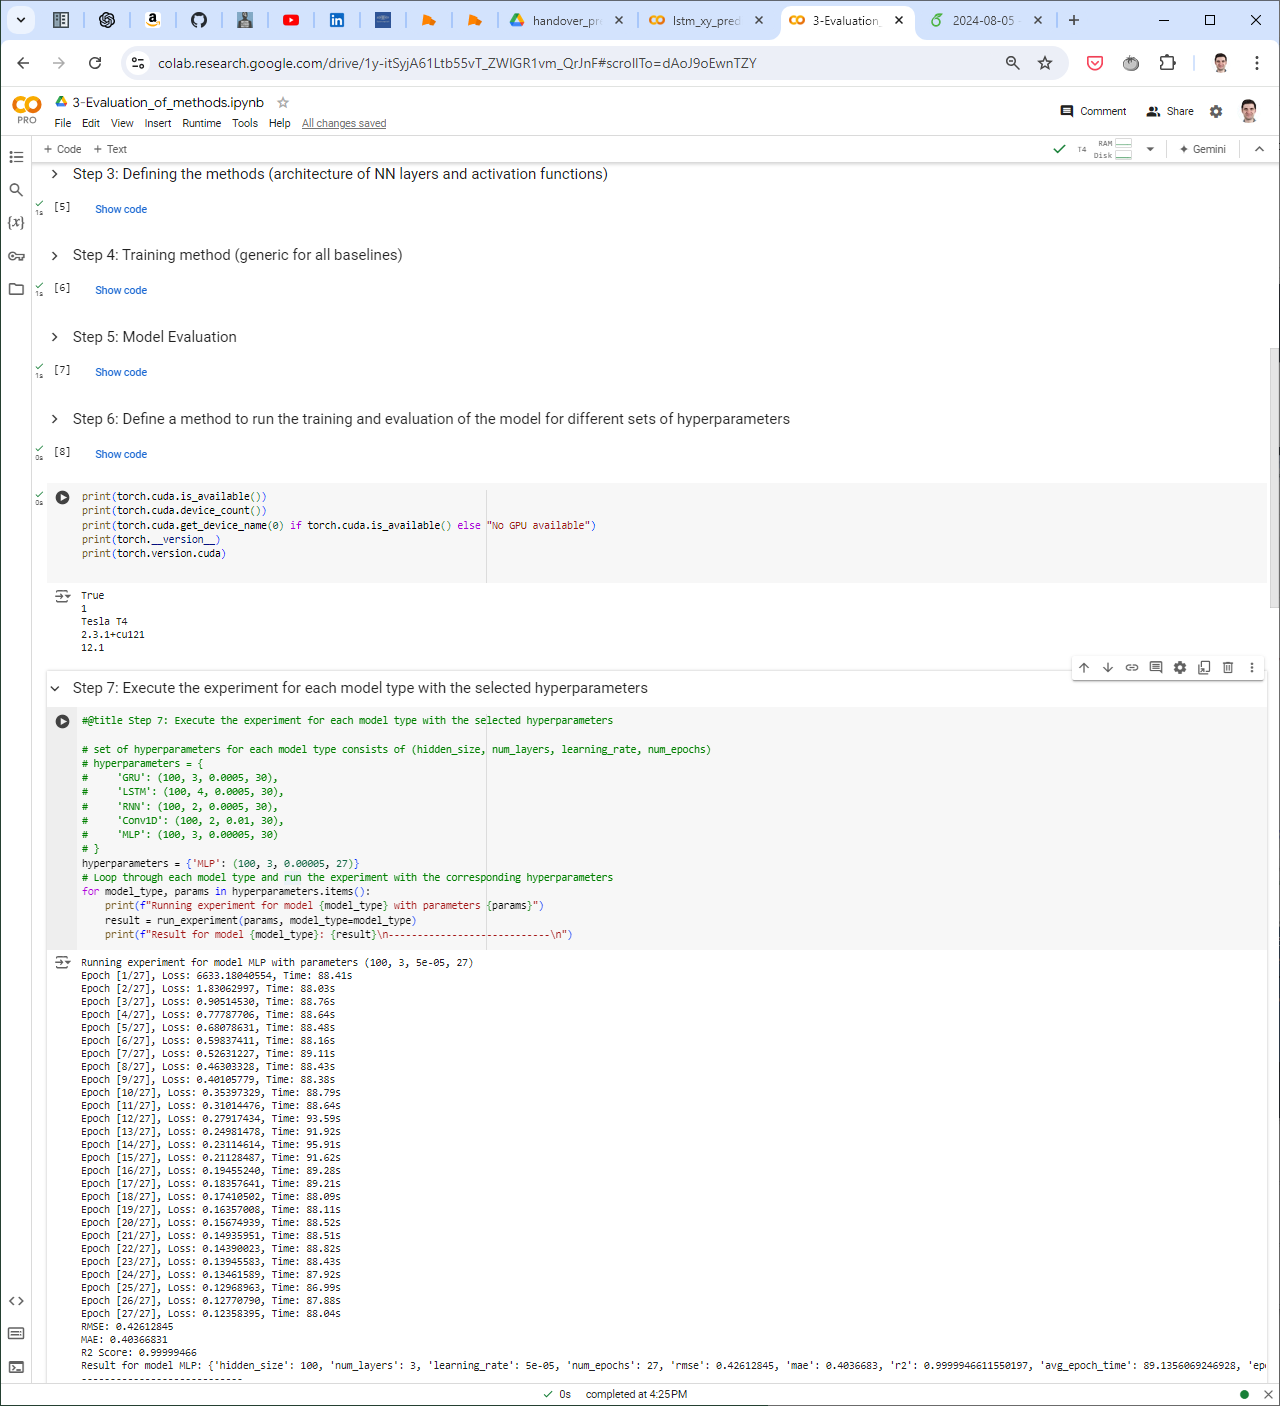
\includegraphics[width=1.01\linewidth]{figures/scr-2-colab.png}
    \caption{Steps 3 to 7: defining the models, training, evaluation, hardware verification, and model execution.}
    \label{fig:scr-2-colab}
\end{figure}

\begin{figure}
    \centering
    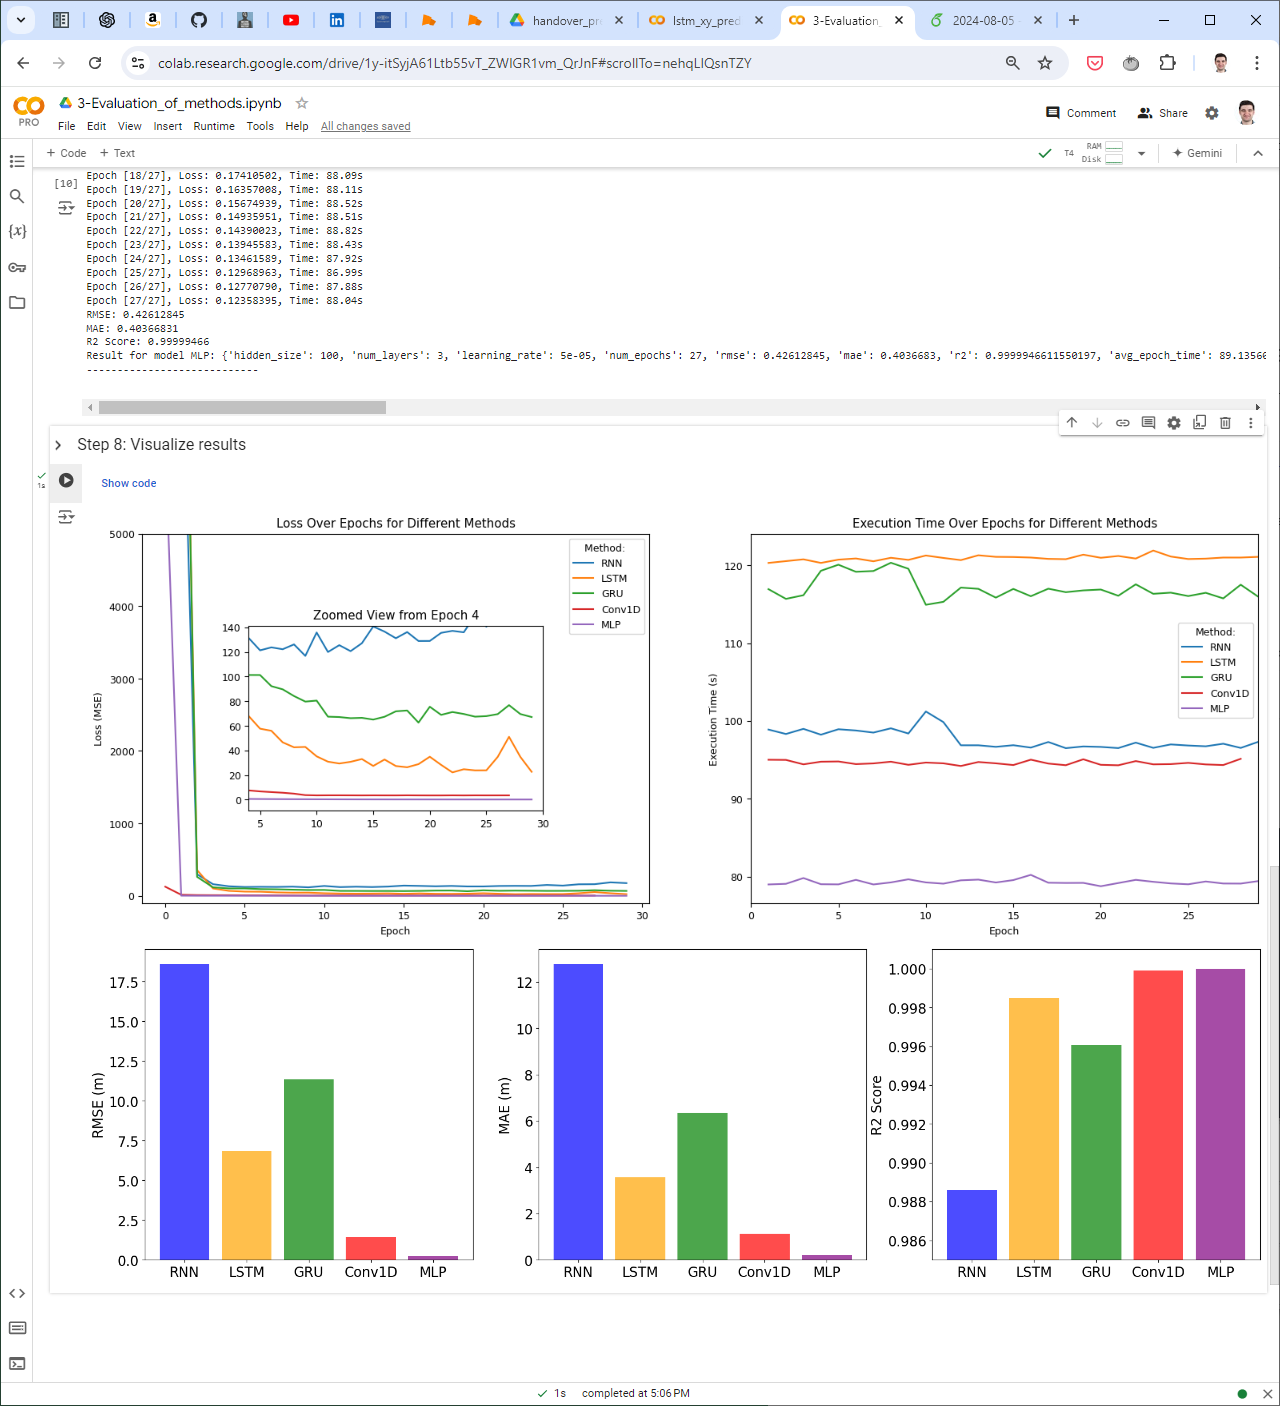
\includegraphics[width=1.01\linewidth]{figures/scr-3-colab.png}
    \caption{Step 8: visualizing different metrics to compare different models.}
    \label{fig:scr-3-colab}
\end{figure}

\begin{figure}
    \centering
    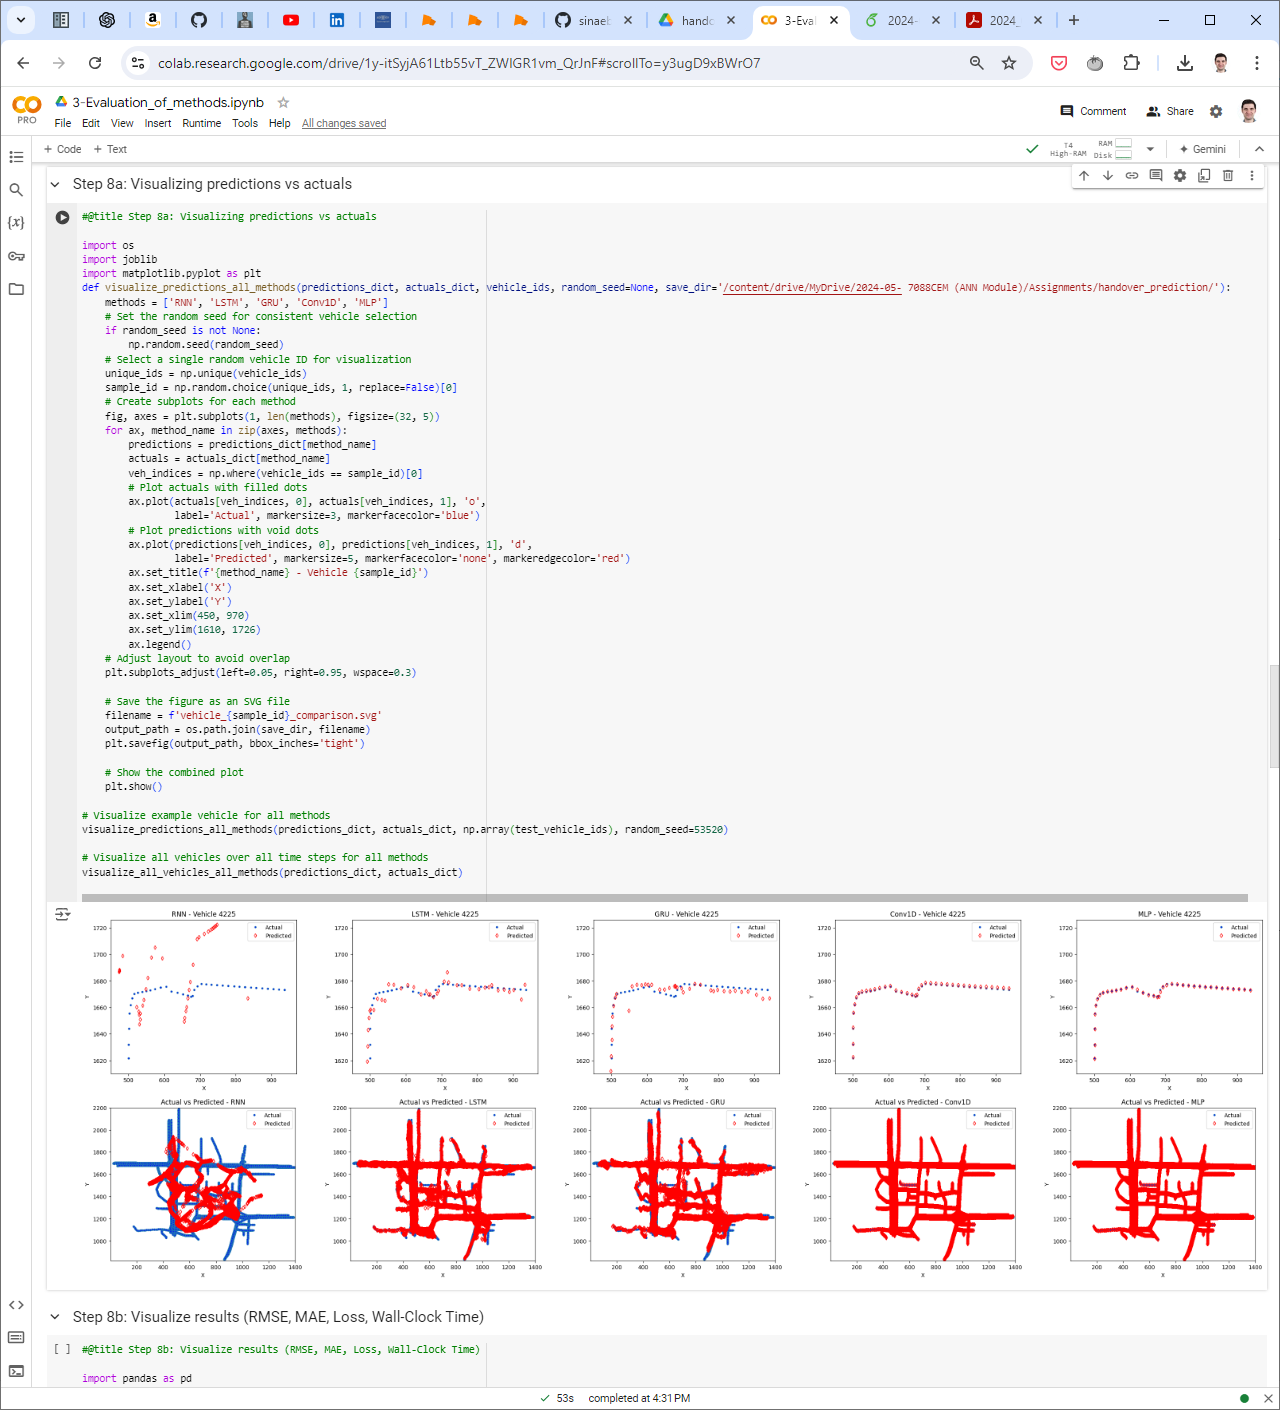
\includegraphics[width=1.01\linewidth]{figures/scr-4-colab.png}
    \caption{Step 8: visualizing predicted and actual locations of vehicles.}
    \label{fig:scr-4-colab}
\end{figure}

%%%%%%%%%%%%%%%%%%%%%%%%%%%%%%%%%%%%%%%%%
\clearpage
\section{Code} \label{appendix-code}
%Appendix 2- Code (10 marks) The complete code in text (in readable format)
One can find the code publicly on a \href{https://github.com/sinaebrahimi/Location_Prediction_-ANN-7088CEM-Project-}{Github repository}. For future use of interested readers, the entire code—including three stages of data preprocessing, hyperparameter tuning, and evaluation of the several approaches—is conveniently compiled here.

\subsection{Preprocessing}\label{preprocessing}
This section presents the steps for preprocessing the file \texttt{OpenStreetMap Trace for a Sparse Traffic.xml}.

% \subsubsection{Convert XML to CSV}
\textbf{1) Convert XML to CSV:}
\begin{minted}[fontsize=\footnotesize, linenos, breaklines, bgcolor=black!5]{python}
import xml.etree.ElementTree as ET
import csv

tree = ET.parse('OpenStreetMap Trace for a Sparse Traffic.xml')
root = tree.getroot()

# open a file for writing
with open('sparse.csv', 'w', newline='') as out_csv:
    writer = csv.writer(out_csv)
    writer.writerow(["time", "id", "x", "y", "angle", "type", "speed", "pos", "lane", "slope"])
    
    for timestep in root.findall('timestep'):
        time = timestep.get('time')
        for vehicle in timestep.findall('vehicle'):
            id = vehicle.get('id')
            x = vehicle.get('x')
            y = vehicle.get('y')
            angle = vehicle.get('angle')
            type = vehicle.get('type')
            speed = vehicle.get('speed')
            pos = vehicle.get('pos')
            lane = vehicle.get('lane')
            slope = vehicle.get('slope')
            writer.writerow([time, id, x, y, angle, type, speed, pos, lane, slope])
\end{minted}

%%%%%%%%%%%%
\textbf{2) Read the input data from the CSV file}
\begin{minted}[fontsize=\footnotesize, linenos, breaklines, bgcolor=black!5]{python}
import pandas as pd

# from google.colab import drive
# drive.mount('/content/drive')

# Load data
data = pd.read_csv('sparse.csv')
# data = pd.read_csv('/content/drive/MyDrive/2024-05- 7088CEM (ANN Module)/Assignments/handover_prediction/sparse.csv')
data.head()
data.info()
data.describe()
\end{minted}

%%%%%%%%%%%%
\textbf{3) Removing the unnecessary columns}
\begin{minted}[fontsize=\footnotesize, linenos, breaklines, bgcolor=black!5]{python}
# Convert the 'time' column to float and then to integer
data['time'] = data['time'].astype(float).astype(int)

# Remove 'veh' from 'id' column and convert to integer
data['id'] = data['id'].str.replace('veh', '').astype(int)

# Remove specified columns
columns_to_remove = ['type', 'lane', 'slope', 'pos']
data = data.drop(columns=columns_to_remove)

# Display the first 10 rows of the processed data
data.head(10)
data.info()
data.describe()

# Save the preprocessed DataFrame to a CSV file for future use
# output_path = '/content/drive/MyDrive/2024-05-7088CEM (ANN Module)/Assignments/handover_prediction/preprocessed_sparse.csv'
output_path = 'preprocessed_sparse.csv'
data.to_csv(output_path, index=False)
print(f"Preprocessed data saved to {output_path}")
\end{minted}

%%%%%%%%%%%%
\textbf{4) Preparing the sequenced data}
In this method, we store a sequence of length 5 for each unique vehicle for the final dataset. This way, the learning algorithm would understand the patterns for the mobility of each vehicle and use it for further prediction. By grouping the vehicles, a total of 1,465,425 sequences were generated from the \texttt{preprocessed\_sparse.csv} file. 

\begin{minted}[fontsize=\footnotesize, linenos, breaklines, bgcolor=black!5]{python}
import pickle

sequence_length = 5

def create_sequences(data, sequence_length):
    sequences = [] # each seqence has the properties of one vehicle in different time steps (sequential)
    vehicle_ids = []
    for veh_id, group in data.groupby('id'):
        group = group.sort_values(by='time')
        for i in range(len(group) - sequence_length):
            seq = group.iloc[i:i+sequence_length]
            sequences.append((seq[['x', 'y', 'speed', 'angle']].values, seq[['x', 'y']].values[-1]))
            vehicle_ids.append(veh_id)
    return sequences, vehicle_ids

sequences, vehicle_ids = create_sequences(data, sequence_length)

# Save sequences to a pkl file
# with open('/content/drive/MyDrive/2024-05- 7088CEM (ANN Module)/Assignments/handover_prediction/sequences_vehicle_ids.pkl', 'wb') as f:
with open('sequences_vehicle_ids.pkl', 'wb') as f:
    pickle.dump((sequences, vehicle_ids), f)
\end{minted}

%%%%%%%%%%%%
\textbf{5) Splitting the dataset into train and test datasets}
We split the data with 80-20\% ratio between train and test datasets.
\begin{minted}[fontsize=\footnotesize, linenos, breaklines, bgcolor=black!5]{python}
import pickle

# Load sequences and vehicle IDs from a file
#with open('/content/drive/MyDrive/2024-05- 7088CEM (ANN Module)/Assignments/handover_prediction/sequences_vehicle_ids.pkl', 'rb') as f:
with open('sequences_vehicle_ids.pkl', 'rb') as f:
    sequences, vehicle_ids = pickle.load(f)

# Split data into training and testing
train_size = int(0.8 * len(sequences))
train_sequences = sequences[:train_size]
test_sequences = sequences[train_size:]
train_vehicle_ids = vehicle_ids[:train_size]
test_vehicle_ids = vehicle_ids[train_size:]

# Define Dataset class
from torch.utils.data import Dataset, DataLoader

class VehicleDataset(Dataset):
    def __init__(self, sequences, flatten=False):
        self.sequences = sequences
        self.flatten = flatten # new

    def __len__(self):
        return len(self.sequences)

    def __getitem__(self, idx):
        seq, target = self.sequences[idx]
        seq_tensor = torch.Tensor(seq)
        if self.flatten:
            seq_tensor = seq_tensor.view(-1)  # Flatten the sequence
        return seq_tensor, torch.Tensor(target)

# Create DataLoader objects for the full dataset
train_dataset_all = VehicleDataset(train_sequences, flatten=False)
test_dataset_all = VehicleDataset(test_sequences, flatten=False)

train_loader_all = DataLoader(train_dataset_all, batch_size=32, shuffle=True)
test_loader_all = DataLoader(test_dataset_all, batch_size=32, shuffle=False)

# Split train dataset for hyperparameter tuning
tune_size = int(0.1 * len(train_sequences))  # Use 10% of the training data for tuning
tune_sequences = train_sequences[:tune_size]
tune_vehicle_ids = train_vehicle_ids[:tune_size]

tune_dataset = VehicleDataset(tune_sequences, flatten=False)
tune_test_size = int(0.1 * len(test_sequences))  # Use 10% of the testing data for tuning
tune_test_sequences = test_sequences[:tune_test_size]

tune_test_dataset = VehicleDataset(tune_test_sequences, flatten=False)

# Create DataLoader objects for tuning set
train_loader = DataLoader(tune_dataset, batch_size=32, shuffle=True)
test_loader = DataLoader(tune_test_dataset, batch_size=32, shuffle=False)
\end{minted}

\clearpage
\subsection{Hyperparameter Tuning} \label{tuning-annex}
In this section, we define our models and hyperparameter grid to execute the experiments in order to choose the best hyperparameters for each method.

%%%%%%%%%%%%
\textbf{1) Import necessary libraries:}
\begin{minted}[fontsize=\footnotesize, linenos, breaklines, bgcolor=black!5]{python}
#@title Step 1: Importing the necessary libraries
import pandas as pd
import numpy as np
import torch
from torch.utils.data import Dataset, DataLoader
import pickle
import time
import itertools
import os
\end{minted}

%%%%%%%%%%%%
\textbf{2) Loading tuning train and test datasets: } We use only 10\% of the data of each datasets for hyperparameter tuning in order to reduce the computation time. For this step, just copy the code from step 5 of Sec. \ref{preprocessing}. \texttt{train\_loader} and \texttt{test\_loader} will be used in the next steps.

%%%%%%%%%%%%
\textbf{3) Defining the methods:} In this section, the architecture of each method and the activation functions between the NN layers are defined.
\begin{minted}[fontsize=\footnotesize, linenos, breaklines, bgcolor=black!5]{python}
#@title Step 3: Defining the methods (architecture of NN layers and activation functions)

#### Step 3a: Define the Long Short-Term Memory (LSTM) model

import torch.nn as nn
import torch.nn.functional as F

class LSTMModel(nn.Module):
    def __init__(self, input_size, hidden_size, num_layers, output_size):
        super(LSTMModel, self).__init__()
        self.hidden_size = hidden_size
        self.num_layers = num_layers
        self.lstm = nn.LSTM(input_size, hidden_size, num_layers, batch_first=True)
        self.fc = nn.Linear(hidden_size, output_size)

    def forward(self, x):
        h0 = torch.zeros(self.num_layers, x.size(0), self.hidden_size).to(x.device)
        c0 = torch.zeros(self.num_layers, x.size(0), self.hidden_size).to(x.device)
        out, _ = self.lstm(x, (h0, c0))
        out = self.fc(out[:, -1, :])
        return out

#### Step 3b: Define the Gated Recurrent Unit (GRU) model

class GRUModel(nn.Module):
    def __init__(self, input_size, hidden_size, num_layers, output_size):
        super(GRUModel, self).__init__()
        self.hidden_size = hidden_size
        self.num_layers = num_layers
        self.gru = nn.GRU(input_size, hidden_size, num_layers, batch_first=True)
        self.fc = nn.Linear(hidden_size, output_size)

    def forward(self, x):
        h0 = torch.zeros(self.num_layers, x.size(0), self.hidden_size).to(x.device)
        out, _ = self.gru(x, h0)
        out = self.fc(out[:, -1, :])
        return out


#### Step 3c: Define the generic Recurrent Neural Network (RNN) model

class RNNModel(nn.Module):
    def __init__(self, input_size, hidden_size, num_layers, output_size):
        super(RNNModel, self).__init__()
        self.hidden_size = hidden_size
        self.num_layers = num_layers
        self.rnn = nn.RNN(input_size, hidden_size, num_layers, batch_first=True)
        self.fc = nn.Linear(hidden_size, output_size)

    def forward(self, x):
        h0 = torch.zeros(self.num_layers, x.size(0), self.hidden_size).to(x.device)
        out, _ = self.rnn(x, h0)
        out = self.fc(out[:, -1, :])
        return out


#### Step 3d: Define 1-d CNN (Conv1D) model

class Conv1DModel(nn.Module):
    def __init__(self, input_size, hidden_size, num_layers, output_size):
        super(Conv1DModel, self).__init__()
        self.conv_layers = nn.ModuleList()
        self.pool_layers = nn.ModuleList()

        # Input layer
        self.conv_layers.append(nn.Conv1d(input_size, hidden_size, kernel_size=3, padding=1))
        self.pool_layers.append(nn.MaxPool1d(kernel_size=2, stride=1))  # Reduced stride

        # Hidden layers
        for _ in range(1, num_layers):
            self.conv_layers.append(nn.Conv1d(hidden_size, hidden_size, kernel_size=3, padding=1))
            self.pool_layers.append(nn.MaxPool1d(kernel_size=2, stride=1))  # Reduced stride

        self.fc = nn.Linear(hidden_size, output_size)

    def forward(self, x):
        x = x.transpose(1, 2)  # Swap dimensions to fit Conv1d input format
        for conv, pool in zip(self.conv_layers, self.pool_layers):
            x = F.relu(conv(x))
            x = pool(x)
        x = x.mean(dim=2)  # Global average pooling
        x = self.fc(x)
        return x
    
#### Step 3e: Define a simple Multi-layer Perceptron (MLP) model

class MLPModel(nn.Module):
    def __init__(self, input_size, hidden_size, num_layers, output_size):
        super(MLPModel, self).__init__()
        layers = [nn.Linear(input_size, hidden_size), nn.ReLU()]

        for _ in range(1, num_layers):
            layers.extend([nn.Linear(hidden_size, hidden_size), nn.ReLU()])

        layers.append(nn.Linear(hidden_size, output_size))
        self.network = nn.Sequential(*layers)

    def forward(self, x):
        return self.network(x.view(x.size(0), -1))
\end{minted}

%%%%%%%%%%%%
\textbf{4) Training: } This section provides a comprehensive approach for training the models. Additionally, a premature termination mechanism is established such that if the training loss does not decrease by more than 1\% in four consecutive epochs, the execution will be halted to conserve computational resources.
\begin{minted}[fontsize=\footnotesize, linenos, breaklines, bgcolor=black!5]{python}
#@title Step 4: Training method (generic for all baselines)

def train_model(model, train_loader, criterion, optimizer, num_epochs=10, device='cuda', early_stopping_rounds=4, min_delta=0.01):
    model.to(device)
    epoch_times = []
    epoch_losses = []

    for epoch in range(num_epochs):
        start_time = time.time()
        model.train()
        total_loss = 0
        for sequences, targets in train_loader:
            sequences, targets = sequences.to(device), targets.to(device)
            outputs = model(sequences)
            loss = criterion(outputs, targets)
            optimizer.zero_grad()
            loss.backward()
            optimizer.step()
            total_loss += loss.item()
        average_loss = total_loss / len(train_loader)
        epoch_time = time.time() - start_time
        epoch_times.append(epoch_time)
        epoch_losses.append(average_loss)
        print(f'Epoch [{epoch+1}/{num_epochs}], Loss: {average_loss:.8f}, Time: {epoch_time:.2f}s')

        # Early stopping mechanism
        if epoch >= early_stopping_rounds:
          recent_losses = epoch_losses[-early_stopping_rounds:]
          if all(abs(recent_losses[i] - recent_losses[i-1]) < min_delta * recent_losses[i-1] for i in range(1, early_stopping_rounds)):
              print(f"Early stopping at epoch {epoch+1}")
              break

    return epoch_times, epoch_losses
\end{minted}

%%%%%%%%%%%%
\textbf{5) Model evaluation: } In this section, we evaluate the trained models with the test dataset with MAE, RMSE, and $\text{R}^2$ score metrics.
\begin{minted}[fontsize=\footnotesize, linenos, breaklines, bgcolor=black!5]{python}
#@title Step 5: Model Evaluation

from sklearn.metrics import mean_absolute_error, r2_score

def evaluate_model(model, test_loader, device='cuda'):
    model.to(device)
    model.eval()
    predictions = []
    actuals = []

    with torch.no_grad():
        for sequences, targets in test_loader:
            sequences, targets = sequences.to(device), targets.to(device)
            outputs = model(sequences)
            predictions.extend(outputs.cpu().numpy())
            actuals.extend(targets.cpu().numpy())

    predictions = np.array(predictions)
    actuals = np.array(actuals)

    # Calculate the metrics
    rmse = np.sqrt(np.mean((predictions - actuals) ** 2))
    mae = mean_absolute_error(actuals, predictions)
    r2 = r2_score(actuals, predictions)

    print(f'RMSE: {rmse:.8f}')
    print(f'MAE: {mae:.8f}')
    print(f'R2 Score: {r2:.8f}')

    return predictions, actuals, rmse, mae, r2
\end{minted}

%%%%%%%%%%%%
\textbf{6) Specify the general procedure for doing each experiment using a single set of hyperparameters: } The MSE is selected as the loss function criterion, and the Adam optimizer is chosen for training optimization.
\begin{minted}[fontsize=\footnotesize, linenos, breaklines, bgcolor=black!5]{python}
#@title Step 6: Define a method to run the training and evaluation of the model for different sets of hyperparameters

def run_experiment(params, input_size=4, output_size=2, model_type='LSTM', save_dir='/content/drive/MyDrive/2024-05- 7088CEM (ANN Module)/Assignments/handover_prediction/'):
    hidden_size, num_layers, learning_rate, num_epochs = params

    if model_type == 'LSTM':
        model = LSTMModel(input_size, hidden_size, num_layers, output_size)
        save_path = 'experiment_results_LSTM.csv'
    elif model_type == 'GRU':
        model = GRUModel(input_size, hidden_size, num_layers, output_size)
        save_path = 'experiment_results_GRU.csv'
    elif model_type == 'RNN':
        model = RNNModel(input_size, hidden_size, num_layers, output_size)
        save_path = 'experiment_results_RNN.csv'
    elif model_type == 'Conv1D':
        model = Conv1DModel(input_size, hidden_size, num_layers, output_size)
        save_path = 'experiment_results_Conv1D.csv'
    elif model_type == 'MLP':
        example_input, _ = next(iter(train_loader))
        flattened_input_size = example_input.view(example_input.size(0), -1).size(1)
        model = MLPModel(flattened_input_size, hidden_size, num_layers, output_size)
        save_path = 'experiment_results_MLP.csv'
    else:
        raise ValueError(f"Unsupported model type: {model_type}")

    # Initialize criterion and optimizer
    criterion = nn.MSELoss() # mean squared error (MSE) is the criterion for evaluating loss in each epoch
    optimizer = torch.optim.Adam(model.parameters(), lr=learning_rate) # Using Adam optimizer

    # Train the model and measure time
    device = 'cuda' if torch.cuda.is_available() else 'cpu'

    #%%%%%%% TRAIN %%%%%%
    # Use the provided train_model function
    epoch_times, epoch_losses = train_model(model, train_loader, criterion, optimizer, num_epochs=num_epochs, device=device)

    # Save the trained model
    model_save_path = os.path.join(save_dir, f'{model_type}_model.pth')
    torch.save(model.state_dict(), model_save_path)
    print(f"Saved {model_type} model to {model_save_path}")
    
    #%%%%%%% TEST %%%%%%
    # Evaluate the model
    predictions, actuals, rmse, mae, r2 = evaluate_model(model, test_loader, device=device)

    # Save predictions and actuals for each method
    data_save_path = os.path.join(save_dir, f'{model_type}_predictions_actuals.pkl')
    with open(data_save_path, 'wb') as f:
        joblib.dump((predictions, actuals), f) 

    # Calculate average epoch time
    avg_epoch_time = np.mean(epoch_times)

    result = {
        'hidden_size': hidden_size,
        'num_layers': num_layers,
        'learning_rate': learning_rate,
        'num_epochs': num_epochs,
        'rmse': rmse,
        'mae': mae,
        'r2': r2,
        'avg_epoch_time': avg_epoch_time,
        'epoch_times': epoch_times,
        'epoch_losses': epoch_losses
    }

    results_df = pd.DataFrame([result])
    if save_path:
        if os.path.exists(save_path):
            results_df.to_csv(save_path, mode='a', header=False, index=False)
        else:
            results_df.to_csv(save_path, index=False)

    return result, predictions, actuals
\end{minted}

%%%%%%%%%%%%
\textbf{7) Define hyperparameter grid and the generic method to run a specific experiment: } The \texttt{run\_specific\_experiment} method allows for the execution of a specific set of hyperparameters, providing flexibility in case the execution is interrupted and needs to be resumed from a previous point. For instance, if the previous execution went up to the 25th set, we would opt to commence the execution of \texttt{run\_specific\_experiment} from the 26th index when we invoke it again.
\begin{minted}[fontsize=\footnotesize, linenos, breaklines, bgcolor=black!5]{python}
#@title Step 7: Define hyperparameter sets

# Define the hyperparameter grid (2*3*8*1 = 48 total possibilities)
param_grid = {
    'hidden_size': [50, 100],
    'num_layers': [2, 3, 4],
    'learning_rate': [0.1, 0.05, 0.01, 0.005, 0.001, 0.0005, 0.0001, 0.00005],
    'num_epochs': [30] 
}

# Create a list of hyperparameter combinations
param_combinations = list(itertools.product(
    param_grid['hidden_size'],
    param_grid['num_layers'],
    param_grid['learning_rate'],
    param_grid['num_epochs']
))

def run_specific_experiment(index, input_size=4, output_size=2, model_type='LSTM'): # allowed number for index: 0-47
    if index < 0 or index >= len(param_combinations):
        raise ValueError("Index out of range")
    
    params = param_combinations[index]

    print('model type: ', model_type)
    print('index of experiment / total number of experiments: ', str(index+1), ' / ',str(len(param_combinations)))
    print('Hyperparameters set (hidden_size, num_layers, learning_rate, num_epochs): ', params)
    result = run_experiment(params, input_size, output_size, model_type)
    print('---------')    
    return result
\end{minted}

%%%%%%%%%%%%
\textbf{8) Execute each method separately: } 
\begin{minted}[fontsize=\footnotesize, linenos, breaklines, bgcolor=black!5]{python}
#@title Step 8: Execute each method (flexible for continuing unfinished experiments)

# We have 48 sets of experiments due to the different values for hyperparameters in param_grid (defined in Step 7)
# I wanted to run each method sequentially. You can run all of them in one loop (it does not matter).
for i in range(48):
    result = run_specific_experiment(index=i, model_type='LSTM')
for i in range(48):
    result = run_specific_experiment(index=i, model_type='GRU')
for i in range(48):
    result = run_specific_experiment(index=i, model_type='RNN')
for i in range(48): 
    result = run_specific_experiment(index=i, model_type='Conv1D')
for i in range(48):
    result = run_specific_experiment(index=i, model_type='MLP')
\end{minted}

%%%%%%%%%%%%
\textbf{9) Choose the best set of hyperparameters for each method: } In this section, we rank sets of hyperparameters for each of the methods according to their RMSE, MAE, $\text{R}^2$ score, average epoch execution time, and loss slope (based on MSE). 
\begin{minted}[fontsize=\footnotesize, linenos, breaklines, bgcolor=black!5]{python}
# Methods to analyze
methods = ["GRU", "LSTM", "RNN", "Conv1D", "MLP"]

# Function to calculate the loss slope (rate of convergence)
def calculate_loss_slope(losses):
    if isinstance(losses, str):
        losses = eval(losses)  # Convert string representation of list back to list
    # Fit a linear model to the loss data (epochs vs loss)
    epochs = np.arange(1, len(losses) + 1)
    slope, _ = np.polyfit(epochs, losses, 1)
    return slope  # Slope of the loss curve

# Function to rank and select the top 3 experiments
def select_top_experiments(df, epoch_time_weight=0.1):
    # Rank based on RMSE (lower is better)
    df['rank_rmse'] = df['rmse'].rank(ascending=True)
    # Rank based on MAE (lower is better)
    df['rank_mae'] = df['mae'].rank(ascending=True)
    # Rank based on R2 (higher is better)
    df['rank_r2'] = df['r2'].rank(ascending=False)
    # Normalize avg_epoch_time to a 0-1 scale
    df['norm_epoch_time'] = (df['avg_epoch_time'] - df['avg_epoch_time'].min()) / (df['avg_epoch_time'].max() - df['avg_epoch_time'].min())
    # Apply a weight to the normalized epoch time
    df['weighted_epoch_time'] = df['norm_epoch_time'] * epoch_time_weight
    # Calculate and rank based on loss slope (more negative slope is better)
    df['loss_slope'] = df['epoch_losses'].apply(calculate_loss_slope)
    df['rank_loss_slope'] = df['loss_slope'].rank(ascending=True) / 10
    
    # Sum the ranks to get a combined score
    df['combined_rank'] = (df['rank_rmse'] + df['rank_mae'] + df['rank_r2'] +
                           df['weighted_epoch_time'] + df['rank_loss_slope'])
    
    # Sort by the combined rank and select the top 3
    top_experiments = df.sort_values('combined_rank').head(10)
    
    return top_experiments
# Dictionary to store results
results = {}

# Iterate over each method and process the corresponding file
for method in methods:
    filepath = f'experiment_results_{method}.csv'
    
    if os.path.exists(filepath):
        df = pd.read_csv(filepath)
        top_experiments = select_top_experiments(df)
        results[method] = top_experiments
    else:
        print(f"File {filepath} not found in the directory.")

# Display the results for each method
for method, top_experiments in results.items():
    print(f"Top 3 experiments for {method}:")
    display(top_experiments)
    print("\n")

# Saving the best results to new CSV files
for method, top_experiments in results.items():
    top_experiments.to_csv(f'top_3_experiments_{method}.csv', index=False)

\end{minted}

\textbf{10) Visualize results to evaluate different hyperparameters: }
\begin{minted}[fontsize=\footnotesize, linenos, breaklines, bgcolor=black!5]{python}
#@title Step 9: Visualize Results to evalate different hyperparameters

import matplotlib.pyplot as plt
import pandas as pd
from mpl_toolkits.axes_grid1.inset_locator import inset_axes

#%%% # Define methods and their specific zoom parameters
methods = {
    'RNN': {},
    'LSTM': {'xlim_rmse': (4.95e-4, 1.05e-3), 'ylim_rmse': (10, 60), 'xlim_r2': (4.95e-4, 1.05e-3), 'ylim_r2': (0.86, 1)},
    'GRU': {'xlim_rmse': (4.95e-4, 1.05e-3), 'ylim_rmse': (10, 28), 'xlim_r2': (4.9e-4, 1.05e-3), 'ylim_r2': (0.975, 0.997)},
    'Conv1D': {'xlim_rmse': (4.9e-5, 1.1e-2), 'ylim_rmse': (0.3, 2.1), 'xlim_r2': (4.9e-5, 1.1e-2), 'ylim_r2': (0.99986, 1)},
    'MLP': {'xlim_rmse': (4.7e-5, 1.3e-2), 'ylim_rmse': (0.4, 2.3), 'xlim_r2': (4.7e-5, 1.3e-2), 'ylim_r2': (0.99987, 1)},
}

#%%% # Set global font
plt.rcParams['font.family'] = 'Times New Roman'
plt.rcParams['font.size'] = 14

#%%% # Loop through methods
for method, zoom_params in methods.items():
    save_path = f'experiment_results_{method}.csv'
    results_df = pd.read_csv(save_path)

    #%%% #------------------- RMSE -------------------#

    # Plot RMSE for different hyperparameters
    plt.figure(figsize=(14, 7))
    for key, grp in results_df.groupby(['hidden_size', 'num_layers']):
        plt.plot(grp['learning_rate'], grp['rmse'], label=f"hidden_size={key[0]}, num_layers={key[1]}")
    plt.xlabel('Learning Rate')
    plt.ylabel('RMSE')
    plt.xscale('log')
    plt.title(f'RMSE for Different Hyperparameter Combinations ({method})')
    plt.legend()

    # Add inset of zoomed region if not RNN
    if method != 'RNN':
        ax_inset = inset_axes(plt.gca(), width='40%', height='27%', loc='center', borderpad=2)
        for key, grp in results_df.groupby(['hidden_size', 'num_layers']):
            ax_inset.plot(grp['learning_rate'], grp['rmse'], label=f"hidden_size={key[0]}, num_layers={key[1]}")
        ax_inset.set_xlim(zoom_params['xlim_rmse'])  # Set the limits for x-axis
        ax_inset.set_ylim(zoom_params['ylim_rmse'])  # Set the limits for y-axis
        ax_inset.set_xscale('log')
        ax_inset.set_title('Zoomed View')
    
    plt.subplots_adjust(left=0.05, right=0.95)
    plt.savefig(f'graphs/rmse-{method.lower()}.svg', bbox_inches='tight')
    plt.show()

    #%%% #------------------- R2 Score -------------------#

    # Plot R2 Score for different hyperparameters
    plt.figure(figsize=(14, 7))
    for key, grp in results_df.groupby(['hidden_size', 'num_layers']):
        plt.plot(grp['learning_rate'], grp['r2'], label=f"hidden_size={key[0]}, num_layers={key[1]}")
    plt.xlabel('Learning Rate')
    plt.ylabel('R2 Score')
    plt.xscale('log')
    plt.title(f'R2 Score for Different Hyperparameter Combinations ({method})')
    plt.legend()

    # Add inset of zoomed region if not RNN
    if method != 'RNN':
        ax_inset = inset_axes(plt.gca(), width='40%', height='27%', loc='center', borderpad=2)
        for key, grp in results_df.groupby(['hidden_size', 'num_layers']):
            ax_inset.plot(grp['learning_rate'], grp['r2'], label=f"hidden_size={key[0]}, num_layers={key[1]}")
        ax_inset.set_xlim(zoom_params['xlim_r2'])  # Set the limits for x-axis
        ax_inset.set_ylim(zoom_params['ylim_r2'])  # Set the limits for y-axis
        ax_inset.set_xscale('log')
        ax_inset.set_title('Zoomed View')

    plt.subplots_adjust(left=0.05, right=0.95)
    plt.savefig(f'graphs/r2-{method.lower()}.svg', bbox_inches='tight')
    plt.show()

    #%%% #------------------- MAE -------------------#

    # # Plot MAE for different hyperparameters
    plt.figure(figsize=(14, 7))
    for key, grp in results_df.groupby(['hidden_size', 'num_layers']):
        plt.plot(grp['learning_rate'], grp['mae'], label=f"hidden_size={key[0]}, num_layers={key[1]}")
    plt.xlabel('Learning Rate')
    plt.ylabel('MAE')
    plt.xscale('log')
    plt.title(f'MAE for Different Hyperparameter Combinations ({method})')
    plt.legend()
    plt.subplots_adjust(left=0.05, right=0.95)
    plt.savefig(f'graphs/mae-{method.lower()}.svg', bbox_inches='tight')
    plt.show()
\end{minted}

%%%%%%
\textbf{11) Analyzing the outcomes for each approach: } Within this section, we will provide the RMSE and $\text{R}^2$ score outcomes for each method. Additionally, we will determine the optimal hyperparameter set for each method.


\paragraph{RNN}
Fig. \ref{fig:rmse-rnn} displays the RMSE metric for the RNN approach using various hyperparameters. The results indicate that selecting a learning rate ($\alpha$) of 0.0005 and employing 2 hidden layers, each containing 100 neurons, yields the minimum RMSE value. Furthermore, Fig. \ref{fig:r2-rnn} shows the coefficient of determination ($\text{R}^2$ score) for the RNN technique using various hyperparameters. The findings indicate that employing a RNN with two hidden layers and 100 neurons yields favorable outcomes when utilizing 0.0005 and 0.001 as $\alpha$. Hence, the hyperparameter set for the RNN method that is deemed optimal is $\alpha=0.0005$ with 2 hidden layers, each consisting of 100 neurons.

\begin{figure}[htbp]
    \centering
    \begin{subfigure}[b]{0.5\linewidth}
        \centering
        \includesvg[width=\textwidth]{figures/rmse-rnn.svg}
        \caption{}
        \label{fig:rmse-rnn}
    \end{subfigure}%
    \begin{subfigure}[b]{0.5\linewidth}
        \centering
        \includesvg[width=\textwidth]{figures/r2-rnn.svg}
        \caption{}
        \label{fig:r2-rnn}
    \end{subfigure}
    \caption{a) RMSE and b) $\text{R}^2$ score of the RNN method with different hyperparameters.}
    \label{fig:rnn-hypers}
\end{figure}

\paragraph{LSTM}
Fig. \ref{fig:rmse-lstm} illustrates the RMSE metric for the LSTM approach with different hyperparameters. The findings suggest that choosing 0.0005 and 0.001 as the values for $\alpha$ and utilizing either 2 hidden layers, each consisting of 100 neurons, results in the lowest RMSE value. Furthermore, Fig. \ref{fig:r2-lstm} displays the $\text{R}^2$ score of the LSTM technique using various hyperparameters. The findings indicate that using a LSTM model with two hidden layers and 100 neurons leads to favorable results when using 0.0005 as $\alpha$. Therefore, the most effective hyperparameter configurations for the LSTM technique includes two layers, with each layer comprising 100 neurons, and a $\alpha$ value of 0.0005.

\begin{figure}[htbp]
    \centering
    \begin{subfigure}[b]{0.5\linewidth}
        \centering
        \includesvg[width=\textwidth]{figures/rmse-lstm.svg}
        \caption{}
        \label{fig:rmse-lstm}
    \end{subfigure}%
    \begin{subfigure}[b]{0.5\linewidth}
        \centering
        \includesvg[width=\textwidth]{figures/r2-lstm.svg}
        \caption{}
        \label{fig:r2-lstm}
    \end{subfigure}
    \caption{a) RMSE and b) $\text{R}^2$ score of the LSTM method with different hyperparameters.}
    \label{fig:lstm-hypers}
\end{figure}

\paragraph{GRU}
Fig. \ref{fig:rmse-gru} displays the RMSE metric for the GRU method across different hyperparameters. The results suggest that selecting 0.0005 as the value of $\alpha$ and using 3 hidden layers, each comprising of 100 neurons, yields the minimum RMSE value. Moreover, Fig. \ref{fig:r2-gru} illustrates the $\text{R}^2$ score for the GRU technique with various hyperparameters. The results suggest that using a GRU with three hidden layers and 100 neurons produces acceptable results when $\alpha$ is set to 0.0005. Therefore, the hyperparameter configuration considered to be the best for the GRU method is $\alpha=0.0005$ with 3 hidden layers, each containing 100 neurons.

\begin{figure}[htbp]
    \centering
    \begin{subfigure}[b]{0.5\linewidth}
        \centering
        \includesvg[width=\textwidth]{figures/rmse-gru.svg}
        \caption{}
        \label{fig:rmse-gru}
    \end{subfigure}%
    \begin{subfigure}[b]{0.5\linewidth}
        \centering
        \includesvg[width=\textwidth]{figures/r2-gru.svg}
        \caption{}
        \label{fig:r2-gru}
    \end{subfigure}
    \caption{a) RMSE and b) $\text{R}^2$ score of the GRU method with different hyperparameters.}
    \label{fig:gru-hypers}
\end{figure}

\paragraph{Conv1D}
Fig. \ref{fig:rmse-conv1d} displays the RMSE metric for the Conv1D method, showcasing its performance across various hyperparameters. The findings indicate that selecting any combination of layers and neurons can yield positive outcomes within the range of $0.00005 \le \alpha \le 0.01$. However, despite the RMSE being fairly similar within this range, the smallest RMSE is observed when $\alpha$ is set to 0.0005, and there are three hidden layers, each consisting of 50 neurons. Furthermore, Fig. \ref{fig:r2-conv1d} illustrates the $\text{R}^2$ score for the Conv1D technique using different hyperparameters. These results also indicate the same conclusion as the RMSE metric, although the experiments (hidden size = 100, no. of layers = 3, $\alpha$ = 0.001), (hidden size = 50, no. of layers = 3, $\alpha$ = 0.01), (hidden size = 100, no. of layers = 2, $\alpha$ = 0.01), and (hidden size = 50, no. of layers = 4, $\alpha$ = 0.005) are nearly identical to the selected set using the RMSE metric. Therefore, we employ a method that utilizes three hidden layers, each consisting of 50 neurons, and a learning rate of $\alpha=0.0005$. 

\begin{figure}[htbp]
    \centering
    \begin{subfigure}[b]{0.5\linewidth}
        \centering
        \includesvg[width=\textwidth]{figures/rmse-conv1d.svg}
        \caption{}
        \label{fig:rmse-conv1d}
    \end{subfigure}%
    \begin{subfigure}[b]{0.5\linewidth}
        \centering
        \includesvg[width=\textwidth]{figures/r2-conv1d.svg}
        \caption{}
        \label{fig:r2-conv1d}
    \end{subfigure}
    \caption{a) RMSE and b) $\text{R}^2$ score of the Conv1D method with different hyperparameters.}
    \label{fig:conv1d-hypers}
\end{figure}

\paragraph{MLP}
Fig. \ref{fig:rmse-mlp} illustrates the RMSE metric for the MLP method across several hyperparameters. The findings indicate that favorable results can be attained by selecting any configuration of layers and neurons within the specified range of $0.00005 \le \alpha \le 0.01$. However, upon closer examination, it is evident that the optimal RMSE may be attained by utilizing only 2 layers, with each layer consisting of 50 neurons, when $\alpha$ is set to 0.001. Furthermore, Fig. \ref{fig:r2-mlp}  displays the $\text{R}^2$ score for the MLP technique with various hyperparameters. These results support the identical conclusion as the RMSE metric. Hence, a learning rate of 0.001, along with 2 hidden layers and 50 neurons, is considered acceptable. However, other configurations, such as those with learning rates of 0.00005 and 0.0001, regardless of their layer count and neuron size, are also very similar to the chosen hyperparameter set.

\begin{figure}[htbp]
    \centering
    \begin{subfigure}[b]{0.5\linewidth}
        \centering
        \includesvg[width=\textwidth]{figures/rmse-mlp.svg}
        \caption{}
        \label{fig:rmse-mlp}
    \end{subfigure}%
    \begin{subfigure}[b]{0.5\linewidth}
        \centering
        \includesvg[width=\textwidth]{figures/r2-mlp.svg}
        \caption{}
        \label{fig:r2-mlp}
    \end{subfigure}
    \caption{a) RMSE and b) $\text{R}^2$ score of the MLP method with different hyperparameters.}
    \label{fig:mlp-hypers}
\end{figure}

%%%%
\clearpage
\subsection{Evaluation of the Various Methods}
In this section, we train the models with 80\% of the dataset and evaluate them by testing 20\% of the data. We use the best hyperparameter set for each of the methods using the ranking in Sec. \ref{tuning-annex} (see the green rows in Table \ref{tab:tuning-values}). 

%%%%%%%%%%%%
\textbf{1) Import necessary libraries:}
\begin{minted}[fontsize=\footnotesize, linenos, breaklines, bgcolor=black!5]{python}
#@title Step 1: Importing the necessary libraries
import pandas as pd
import numpy as np
import torch
from torch.utils.data import Dataset, DataLoader
import pickle
import time
import itertools
import os
\end{minted}

%%%%%%%%%%%%
\textbf{2) Load preprocessed (sequenced) data; Splitting data into training and testing datasets}
\begin{minted}[fontsize=\footnotesize, linenos, breaklines, bgcolor=black!5]{python}
#@title Step 2: Load preprocessed (sequenced) data; Splitting data into training and testing datasets

# Load sequences and vehicle IDs from a file
with open('sequences_vehicle_ids.pkl', 'rb') as f:
#with open('sequences_vehicle_ids.pkl', 'rb') as f:
    sequences, vehicle_ids = pickle.load(f)

# Split data into training and testing
train_size = int(0.8 * len(sequences))
train_sequences = sequences[:train_size]
test_sequences = sequences[train_size:]
train_vehicle_ids = vehicle_ids[:train_size]
test_vehicle_ids = vehicle_ids[train_size:]

class VehicleDataset(Dataset):
    def __init__(self, sequences, flatten=False):
        self.sequences = sequences
        self.flatten = flatten # new

    def __len__(self):
        return len(self.sequences)

    def __getitem__(self, idx):
        seq, target = self.sequences[idx]
        seq_tensor = torch.Tensor(seq)
        if self.flatten:
            seq_tensor = seq_tensor.view(-1)  # Flatten the sequence
        return seq_tensor, torch.Tensor(target)

# Create DataLoader objects for the full dataset
train_dataset_all = VehicleDataset(train_sequences, flatten=False)
test_dataset_all = VehicleDataset(test_sequences, flatten=False)

train_loader = DataLoader(train_dataset_all, batch_size=32, shuffle=True)
test_loader = DataLoader(test_dataset_all, batch_size=32, shuffle=False)
\end{minted}

%%%%%%%%%%%%
\textbf{3) Defining the methods (models): } We replicate the exact code from step 3 in Sec. \ref{tuning-annex}.

%%%%%%%%%%%%
\textbf{4) Train the model: } We replicate the exact code from step 4 in Sec. \ref{tuning-annex}.

%%%%%%%%%%%%
\textbf{5) Model evaluation: } We replicate the exact code from step 5 in Sec. \ref{tuning-annex}.

%%%%%%%%%%%%
\textbf{6) Specify the general procedure for doing each experiment using a single set of hyperparameters: } We replicate the exact code from step 6 in Sec. \ref{tuning-annex}.

%%%%%%%%%%%%
\textbf{7) Execute each method separately for the selected hyperparameters: }
\begin{minted}[fontsize=\footnotesize, linenos, breaklines, bgcolor=black!5]{python}
#@title Step 7: Execute the experiment for each model type with the selected hyperparameters

# set of hyperparameters for each model type consists of (hidden_size, num_layers, learning_rate, num_epochs)
hyperparameters = {
    'RNN': (100, 2, 0.0005, 10),
    'LSTM': (100, 4, 0.0005, 30),
    'GRU': (100, 3, 0.0005, 15),
    'Conv1D': (100, 2, 0.01, 10),
    'MLP': (100, 3, 0.00005, 10)
}

# Create dictionaries to store predictions and actuals for each model
predictions_dict = {}
actuals_dict = {}

# Loop through each model type and run the experiment with the corresponding hyperparameters
for model_type, params in hyperparameters.items():
    print(f"Running experiment for model {model_type} with parameters {params}")
    result, predictions, actuals = run_experiment(params, model_type=model_type)

    # Store the predictions, actuals, and model save path
    predictions_dict[model_type] = predictions
    actuals_dict[model_type] = actuals

    print(f"Result for model {model_type}: {result}\n----------------------------\n")
\end{minted}

%%%%%%%%%%%%
\textbf{8) Visualize episodic loss and execution time of the methods, along with RMSE, MAE, and $\text{R}^2$ score of their final epoch: }
\begin{minted}[fontsize=\footnotesize, linenos, breaklines, bgcolor=black!5]{python}
import pandas as pd
import matplotlib.pyplot as plt
import ast
from mpl_toolkits.axes_grid1.inset_locator import inset_axes

# Load the CSV file
file_path = 'experiment_methods.csv'
df = pd.read_csv(file_path)

# Convert the 'epoch_losses' column from a string representation of a list to an actual list
df['epoch_losses'] = df['epoch_losses'].apply(ast.literal_eval)

# Set global font to Times New Roman and size to 18
plt.rcParams['font.family'] = 'Times New Roman'
plt.rcParams['font.size'] = 18

# Main plot
plt.figure(figsize=(12, 8))
for index, row in df.iterrows():
    plt.plot(row['epoch_losses'], label=row['method_type'])

plt.xlabel('Epoch')
plt.ylabel('Loss (MSE)')
plt.ylim(-100, 5000)
plt.title('Loss Over Epochs for Different Methods')
plt.legend(title="Method: ", prop={'size': 18})

# Add inset of zoomed region
ax_inset = inset_axes(plt.gca(), width='58%', height='50%', loc='center', borderpad=6)
for index, row in df.iterrows():
    # Starting from epoch 4
    ax_inset.plot(range(4, len(row['epoch_losses'])), row['epoch_losses'][4:], label=row['method_type'])

ax_inset.set_xlim(4, len(df.iloc[0]['epoch_losses']) )
ax_inset.set_ylim(-9, 141)
ax_inset.set_title('Zoomed View from Epoch 4')

plt.savefig('graphs/loss-over-epochs.svg', bbox_inches='tight')
plt.show()

#%%% Execution time:

# Manually extracted execution times from notebook output (from the printed output (it wasn't in the CSV files (only the avg exec time is in the CSV output)))
execution_times = {
    'RNN': [98.89, 98.32, 98.98, 98.23, 98.93, 98.77, 98.50, 99.05, 98.38, 101.21,
            99.85, 96.87, 96.87, 96.67, 96.88, 96.57, 97.29, 96.50, 96.72, 96.66,
            96.51, 97.21, 96.54, 96.98, 96.84, 96.74, 97.07, 96.53, 97.31, 96.26],
    'LSTM': [120.30, 120.53, 120.76, 120.30, 120.72, 120.87, 120.51, 120.96, 120.69, 121.25,
             120.94, 120.66, 121.28, 121.08, 121.06, 120.99, 120.82, 120.78, 121.36, 120.96,
             121.19, 120.86, 121.89, 121.12, 120.80, 120.85, 120.99, 120.99, 121.08, 120.71],    
    'GRU': [116.93, 115.68, 116.15, 119.29, 120.07, 119.16, 119.26, 120.32, 119.55, 114.92,
            115.30, 117.13, 116.97, 115.84, 116.96, 116.02, 116.99, 116.54, 116.77, 116.88,
            116.08, 117.55, 116.33, 116.48, 116.04, 116.46, 115.74, 117.50, 115.96, 116.76],
    'Conv1D': [95.01, 94.99, 94.42, 94.76, 94.79, 94.45, 94.54, 94.76, 94.36, 94.65,
               94.55, 94.21, 94.72, 94.55, 94.33, 95.02, 94.52, 94.31, 95.07, 94.36,
               94.30, 94.84, 94.42, 94.45, 94.61, 94.41, 94.33, 95.13],
    'MLP': [78.99, 79.07, 79.81, 79.02, 79.00, 79.58, 78.99, 79.25, 79.65, 79.25,
            79.09, 79.52, 79.61, 79.24, 79.55, 80.22, 79.21, 79.18, 79.19, 78.76,
            79.17, 79.58, 79.33, 79.12, 79.01, 79.37, 79.11, 79.10, 79.42, 78.87]
}

# Plotting Execution Time for Each Epoch
plt.figure(figsize=(14, 8))

for method, times in execution_times.items():
    plt.plot(range(1, len(times) + 1), times, label=method)

plt.xlabel('Epoch')
plt.xlim(1, 30)
plt.ylabel('Execution Time (s)')
plt.title('Execution Time Over Epochs for Different Methods')
plt.legend(title="Method:", prop={'size': 16}, loc='center right', bbox_to_anchor=(1, 0.63))
# plt.grid(True)
plt.savefig('graphs/exec-time-per-epoch.svg')
plt.show()

#%% RMSE, MAE, and R2 score of the final epoch

# Load the CSV file
file_path = 'experiment_methods.csv'
df = pd.read_csv(file_path)

# Extract the metrics
methods = df['method_type']
rmse_values = df['rmse']
mae_values = df['mae']
r2_values = df['r2']

# Define the original color mapping
color_mapping = {
    'RNN': 'blue',
    'LSTM': 'orange',
    'GRU': 'green',
    'Conv1D': 'red',
    'MLP': 'purple'
}

# Lighten the colors
def lighten_color(color, amount=0.7):
    return to_rgba(color, alpha=amount)

# Apply lighter colors
light_colors = [lighten_color(color_mapping[method], amount=0.7) for method in methods]

# Plotting RMSE, MAE, R2 for each method as a bar plot
plt.rcParams['font.size'] = 17
fig, ax = plt.subplots(1, 3, figsize=(25, 7))

ax[0].bar(methods, rmse_values, color=light_colors)
ax[0].set_ylabel('RMSE (m)')

ax[1].bar(methods, mae_values, color=light_colors)
ax[1].set_ylabel('MAE (m)')

ax[2].bar(methods, r2_values, color=light_colors)
ax[2].set_ylabel('R2 Score')
ax[2].set_ylim(0.985, 1.001)  # Limit the y-axis from 0.985 to 1.001

plt.savefig('graphs/rmse-mae-r2score-methods.svg')
plt.show()
\end{minted}

%%%%%%%%%%%%
\textbf{9) Visualizing predictions vs actuals}
\begin{minted}[fontsize=\footnotesize, linenos, breaklines, bgcolor=black!5]{python}
#@title Step 8a: Visualizing predictions vs actuals

import os
import joblib
import matplotlib.pyplot as plt
import numpy as np

def load_predictions_actuals(method_name, save_dir):
    data_save_path = os.path.join(save_dir, f'{method_name}_predictions_actuals.pkl')
    if os.path.exists(data_save_path):
        with open(data_save_path, 'rb') as f:
            predictions, actuals = joblib.load(f)
        return predictions, actuals
    else:
        raise FileNotFoundError(f"Data for {method_name} not found in {save_dir}.")

def visualize_predictions_all_methods(predictions_dict, actuals_dict, vehicle_ids, random_seed=None, save_dir='/content/drive/MyDrive/2024-05- 7088CEM (ANN Module)/Assignments/handover_prediction/'):
    methods = ['RNN', 'LSTM', 'GRU', 'Conv1D', 'MLP']

    # Load data if predictions_dict and actuals_dict are empty
    if not predictions_dict or not actuals_dict:
        for method in methods:
            try:
                predictions_dict[method], actuals_dict[method] = load_predictions_actuals(method, save_dir)
            except FileNotFoundError as e:
                print(e)
                return

    # Set the random seed for consistent vehicle selection
    if random_seed is not None:
        np.random.seed(random_seed)
    
    # Select a single random vehicle ID for visualization
    unique_ids = np.unique(vehicle_ids)
    sample_id = np.random.choice(unique_ids, 1, replace=False)[0]

    # Create subplots for each method
    fig, axes = plt.subplots(1, len(methods), figsize=(25, 5))
    
    for ax, method_name in zip(axes, methods):
        predictions = predictions_dict[method_name]
        actuals = actuals_dict[method_name]
        
        veh_indices = np.where(vehicle_ids == sample_id)[0]
        
        # Plot actuals with filled dots
        ax.plot(actuals[veh_indices, 0], actuals[veh_indices, 1], 'o',
                label='Actual', markersize=3, markerfacecolor='blue')

        # Plot predictions with void dots
        ax.plot(predictions[veh_indices, 0], predictions[veh_indices, 1], 'd',
                label='Predicted', markersize=5, markerfacecolor='none', markeredgecolor='red')

        ax.set_title(f'{method_name} - Vehicle {sample_id}')
        ax.set_xlabel('X')
        ax.set_ylabel('Y')
        ax.set_xlim(470, 700)
        ax.set_ylim(840, 1670)
        ax.legend()
    
    # Adjust layout to avoid overlap
    plt.subplots_adjust(left=0.05, right=0.95, wspace=0.3)

    # Save the figure as an SVG file
    filename = f'vehicle_{sample_id}_comparison.svg'
    output_path = os.path.join(save_dir, filename)
    plt.savefig(output_path, bbox_inches='tight')

    # Show the combined plot
    plt.show()

def visualize_all_vehicles_all_methods(predictions_dict, actuals_dict, save_dir='/content/drive/MyDrive/2024-05- 7088CEM (ANN Module)/Assignments/handover_prediction/'):
    methods = ['RNN', 'LSTM', 'GRU', 'Conv1D', 'MLP']

    # Load data if predictions_dict and actuals_dict are empty
    if not predictions_dict or not actuals_dict:
        for method in methods:
            try:
                predictions_dict[method], actuals_dict[method] = load_predictions_actuals(method, save_dir)
            except FileNotFoundError as e:
                print(e)
                return

    # Create subplots for each method
    fig, axes = plt.subplots(1, len(methods), figsize=(20, 5))

    for ax, method_name in zip(axes, methods):
        predictions = predictions_dict[method_name]
        actuals = actuals_dict[method_name]

        # Plot actuals with filled dots
        ax.plot(actuals[:, 0], actuals[:, 1], 'o',
                label='Actual', markersize=3, markerfacecolor='blue')

        # Plot predictions with void dots
        ax.plot(predictions[:, 0], predictions[:, 1], 'd',
                label='Predicted', markersize=5, markerfacecolor='none', markeredgecolor='red')

        ax.set_title(f'Actual vs Predicted - {method_name}')
        ax.set_xlabel('X')
        ax.set_ylabel('Y')
        ax.set_xlim(2, 1400)
        ax.set_ylim(820, 2200)
        ax.legend()

    # Adjust layout to avoid overlap
    plt.subplots_adjust(left=0.05, right=0.95, wspace=0.3)

    # Save the figure as an SVG file
    filename = 'all_vehicles_comparison.svg'
    output_path = os.path.join(save_dir, filename)
    plt.savefig(output_path, bbox_inches='tight', dpi=100)

    # Show the combined plot
    plt.show()

# Visualize example vehicle for all methods
visualize_predictions_all_methods(predictions_dict, actuals_dict, np.array(test_vehicle_ids), random_seed=3520)

# Visualize all vehicles over all time steps for all methods
visualize_all_vehicles_all_methods(predictions_dict, actuals_dict)
\end{minted}

% \textbf{11) }
% \begin{minted}[fontsize=\footnotesize, linenos, breaklines, bgcolor=black!5]{python}
% \end{minted}
%%%%%%%%%%%%%%%%%%%%%%%%%%%%%%%%%%%%%%%%%
\end{appendices}

\end{document}
